\documentclass{ceurart}

\usepackage{acronym}
\usepackage{subcaption}
\usepackage{listings}
\usepackage[section]{placeins}

\renewcommand{\acffont}[1]{\textsl{#1}}


%%
%% end of the preamble, start of the body of the document source.
\begin{document}

%%
%% Rights management information.
%% CC-BY is default license.
\copyrightyear{2023}
\copyrightclause{Copyright for this paper by its authors.\\
  Use permitted under Creative Commons License Attribution 4.0
  International (CC BY 4.0).}

%%
%% This command is for the conference information
\conference{CLEF 2023: Conference and Labs of the Evaluation Forum, September 18--21, 2023, Thessaloniki, Greece}

%%
%% The "title" command
\title{SEUPD@CLEF: Team FADERIC on A Query Expansion and Reranking Approach for the Longeval Task}

\title[mode=sub]{Notebook for the LongEval Lab at CLEF 2023}

%%
%% The "author" command and its associated commands are used to define
%% the authors and their affiliations.
\author[1]{Enrico Bolzonello}[%
email=enrico.bolzonello@studenti.unipd.it
]

\author[1]{Christian Marchiori}[%
email=christian.marchiori@studenti.unipd.it
]

\author[1]{Daniele Moschetta}[%
email=daniele.moschetta@studenti.unipd.it
]

\author[1]{Riccardo Trevisiol}[%
email=riccardo.trevisiol.1@studenti.unipd.it
]

\author[1]{Fabio Zanini}[%
email=fabio.zanini@studenti.unipd.it
]

\author[1]{Nicola Ferro}[%
orcid=0000-0001-9219-6239,
email=ferro@dei.unipd.it,
url=http://www.dei.unipd.it/~ferro/,
]


\address[1]{University of Padua, Italy}


%%
%% The abstract is a short summary of the work to be presented in the
%% article.
\begin{abstract}
This report explains and analyzes the system developed by Team FADERIC for the LongEval Lab at CLEF 2023, Task 1 - LongEval-Retrieval. The team members are all students following the Search Engines course a.y. 2022/23 at the Computer Engineering master degree at University of Padua. The system developed is a search engine that has to retrieve documents from a corpus, composed of original files in French language and automatically translated files in English language. The produced IR system exploits the query expansion technique, such as word N-grams and synonyms, and also the use of a reranking to improve the overall performance. Evaluating the longitudinal effectiveness of the system using the multiple collections provided by CLEF, we show that the performances remain satisfactory over time.
\end{abstract}

%%
%% Keywords. The author(s) should pick words that accurately describe
%% the work being presented. Separate the keywords with commas.
\begin{keywords}
	CLEF \sep
	LongEval \sep
	Information retrieval \sep
	Search engines \sep
	Query expansion \sep
	Reranking
\end{keywords}

%%
%% This command processes the author and affiliation and title
%% information and builds the first part of the formatted document.
\maketitle


\section{Introduction}
\label{sec:introduction}

Search engines have become an indispensable tool for people to retrieve various kinds of information in their daily 
routine. However, recent research has shown that \ac{IR} systems tend to perform poorly over time as the test data becomes more distant from the training data. This issue is particularly critical in the field of computer science, where data is constantly updated and information quickly becomes obsolete. Therefore, \ac{CLEF} 2023 LongEval task \cite{longevaloverview2023} has gained interest in evaluating the temporal persistence of \ac{IR} systems. The aim of this report is to present the solution of Team FADERIC to this challenge. The team members are all students following the Search Engines course a.y. 2022/23 at the Computer Engineering master degree at University of Padua. \\The paper is organized as follows: Section~\ref{sec:related} shows the related work we have started from; Section~\ref{sec:methodology} describes our approach; Section~\ref{sec:setup} explains our experimental setup; Section~\ref{sec:results} discusses our main findings; finally, Section~\ref{sec:conclusion} draws some conclusions and outlooks for future work.

\section{Related Work}
\label{sec:related}

To understand the task and the collections provided by \ac{CLEF} we have used the paper by LongEval organizers \citet{galuvsvcakova2023longeval}. This has helped us to tackle the problem by figuring out how given documents and queries were collected and which were the main goals of the task. In the paper are also given some \emph{baseline} performances that we have used to benchmark our system during its development. 

We decided to exploit query expansion techniques basing our knowledge of the theme on the works from \citet{carpineto2012survey} and \citet{azad2019query}. We have decided to use various techniques, such as word N-grams and synonyms, which we have then tried during the development of our system.

Moreover, we choose to approach the problem by also using \emph{reranking}. To do so we have used the work from \citet{alkhalifa2022building}, which explains the problem of using a language model to address the longitudinal evaluation task. We build our reranking approach based on the work from \citet{Birch} who developed the Birch system.

\section{Methodology}
\label{sec:methodology}

In this section, we describe the methodology we have adopted in order to develop an \ac{IR} system for the task.

\subsection{Parser}
\label{subsec:parser}

%%brief parser description
We manually inspected the documents provided by \ac{CLEF} in order to understand their \emph{structure} and be able to extract the body and ID of each document from them.

In order to do that, we created a tool called \emph{parser} that has been essential for extracting information from documents in the specified format 
used by \ac{TREC}. The parser helps us create structured objects that are used for analysis and indexing within the \ac{IR} system.

Here are the key components we implemented:
\begin{itemize}
    \item  \textbf{\texttt{ParsedDocument}}: represents a parsed document to be indexed.  It has two attributes: \texttt{ID} for the unique identifier of the document and \texttt{body} for the document's content. This class provides functionalities to set and retrieve documents' attributes.
    \item  \textbf{\texttt{DocumentParser}}: represents an abstract class providing basic functionalities to iterate over the elements of a \texttt{ParsedDocument}, reading and parsing its content.

    \item  \textbf{\texttt{LongEvalDocumentParser}}: specific \texttt{DocumentParser} for the LongEval corpus. It provides an implementation of a parser for the documents in the TREC format. The parser reads a document and returns a \texttt{ParsedDocument} that contains the \texttt{ID} and the \texttt{body} of the document.
\end{itemize}   

We used  the \texttt{LongEvalDocumentParser} and the \texttt{ParsedDocument} in the indexer to represent the content of the documents that are 
in the directory specified by \texttt{docsDir}. The first one has been used to iterate over the content of the specified document, while the second one has been used to represent a document to be indexed.
\newpage
\subsection{Analyzer}
\label{subsec:analyzer}

In order to \emph{process texts} from documents and queries, we have implemented custom analyzers: since the collections are provided in both French and English language, two of them have been implemented.

\subsubsection{French analyzer}

The \texttt{FrenchLongEvalAnalyzer} component is in charge of processing French language texts, it is composed by:
\begin{itemize}
    \item \textbf{Tokenizing}: the \texttt{StandardTokenizer} is used, which exploits the Word Break rules from Unicode Text Annex \#29 \citep{UAX29};
    \item \textbf{Character folding}: the \texttt{ICUFoldingFilter} is used, which applies the foldings from Unicode Technical Report \#30 \citep{UTR30}. This is useful to fold upper cases, accents and other kinds of complex characters;
    \item \textbf{Elision removal}: the \texttt{ElisionFilter} is used, which removes the elision from words;
    \item \textbf{Stopword removal}: the \texttt{StopFilter} is used, which removes the given stopwords from the tokens. In this system we have tried using the default Lucene \citep{Lucene} stoplist and custom one, generated by picking the 50 most frequent terms in the documents;
    \item \textbf{Position filtering}: a custom \texttt{TokenFilter} has been implemented to set the \texttt{positionIncrement} attribute of all tokens to a specific value. This will be useful to ignore the \texttt{positionIncrement} due to removed stopwords in the search phase when we will use the proximity between tokens, as explained in Subsection~\ref{subsubsec:shingles};
    \item \textbf{Stemming}: this process is useful to reduce words to their base form, in this system we have tried using the Snowball French \citep{FrSnowball} and Light \citep{LightStem} stemmers.
\end{itemize}

In Table~\ref{tab:french-analyzer} we show an example of the analyzing process for the French language.

\begin{table}[b]
    \caption{French analyzer process}
    \label{tab:french-analyzer}
    \centering
    \begin{tabular}{|c|c|}
        \toprule
        \textbf{Step} & \textbf{Tokens}\\
        \midrule
          & La méthode d'analyse de texte est\\ 
          & essentielle pour l'extraction d'informations.\\ 
         \midrule
         Tokenizing & [La, méthode, d'analyse, de, texte, est,\\
         & essentielle, pour, l'extraction, d'informations]\\
         \midrule
         Character folding & [la, methode, d'analyse, de, texte, est,\\
          & essentielle, pour, l'extraction, d'informations]\\
         \midrule
         Stopword removal & [methode, analyse, texte,\\
         (50 most freq.) & essentielle, extraction, informations]\\
         \midrule
         Stemming & [method, analys, text,\\
         (Ligth) & esentiel, extraction, inform]\\
        \bottomrule
    \end{tabular}
\end{table}

\subsubsection{English analyzer}

The \texttt{EnglishLongEvalAnalyzer} component is in charge of processing English language texts, it is composed by:
\begin{itemize}
    \item \textbf{Tokenizing}: the \texttt{StandardTokenizer} is used, which exploits the Word Break rules from Unicode Text Annex \#29 \citep{UAX29};
    \item \textbf{Character folding}: the \texttt{ICUFoldingFilter} is used, which applies the foldings from Unicode Technical Report \#30 \citep{UTR30}. This is useful to fold upper cases, accents and other kinds of complex characters;
    \item \textbf{Possessive removal}: the \texttt{EnglishPossessiveFilter} is used, which removes the very frequent possessives ('s) from words;
    \item \textbf{Stopword removal}: the \texttt{StopFilter} is used, which removes the given stopwords from the tokens. In this system we have tried using the default Lucene \citep{Lucene} stoplist and custom one, generated by picking the 50 most frequent terms in the documents;
    \item \textbf{Position filtering}: a custom \texttt{TokenFilter} has been implemented to set the \texttt{positionIncrement} attribute of all tokens to a specific value. This will be useful to ignore the \texttt{positionIncrement} due to removed stopwords in the search phase when we will use the proximity between tokens, as explained in Subsection~\ref{subsubsec:shingles};
    \item \textbf{Stemming}: this process is useful to reduce words to their base form, in this system we have tried using the Snowball English (Porter2) \citep{EnSnowball} and the Krovetz \citep{Krovetz2000} stemmers.
\end{itemize}

In Table~\ref{tab:english-analyzer} we show an example of the analyzing process for the English language.

\begin{table}[b]
    \caption{English analyzer process}
    \label{tab:english-analyzer}
    \centering
    \begin{tabular}{|c|c|}
        \toprule
        \textbf{Step} & \textbf{Tokens}\\
        \midrule
        & The text analysis method's importance\\
        & lies in its role in information extraction.\\ 
        \midrule
        Tokenizing & [the, text, analysis, method, importance,\\
        & lies, in, its, role, in, information, extraction]\\
        \midrule
        Character folding & [the, text, analysis, method, importance,\\
        & lies, in, its, role, in, information, extraction]\\
        \midrule
        Stopword removal & [text, analysis, method, importance,\\
        (50 most freq.) & lies, role, information, extraction]\\
        \midrule
        Stemming & [text, analysis, method, importance,\\
        (Krovetz) & lie, role, information, extraction]\\
        \bottomrule
    \end{tabular}
\end{table}
\newpage
\subsection{Indexer}
\label{subsec:indexer}

Indexing is a crucial step where we create a searchable database, called \emph{index}, for the parsed documents. The index contains important information about the documents, 
such as the words and phrases they contain, their frequency, and their location within the document. 
Indexing allows us to store the documents in a \emph{structured} manner, which greatly speeds up the retrieval process by enabling users to search for documents based on keywords or phrases. To achieve this, we developed the following components:

\begin{itemize}
    \item \textbf{\texttt{DirectoryIndexer}}: indexes the documents located in a specified directory and its sub-directories. It accepts various parameters, including the directory containing the documents to be indexed, the \texttt{DocumentParser}, the \texttt{Analyzer}, the \texttt{Similarity} to be used for indexing, the expected number of documents and the location where the index will be stored. Our code ensures that the document directory is readable and the index directory is writable before initiating the indexing process. Additionally, it keeps track of statistics, such as the number of indexed files and documents. \\
The main component of the class is the \texttt{index} method, which is in charge of performing the actual indexing of the documents. This method iterates through the documents in the directory, extracting their content and adding it to the index. During all the iterations, some statistics indexing is given, such as the time taken every 10 thousand documents. Finally, the index is closed.
    \item \textbf{\texttt{BodyField}}: represents the body field of a document. This field has the following properties:

\begin{itemize}
	\item it is \emph{tokenized}, meaning that the body is broken into words, or tokens, to make the search more accurate and flexible;
	\item \emph{frequencies} and also the \emph{positions} of the tokens are stored, in order to allow for phrase queries with proximity, as explained in Section~\ref{subsubsec:shingles};
	\item the body content is \emph{stored}, even if this had an impact on the index size, this was needed in the search phase in order to pass documents bodies to the reranker, as explained in Section~\ref{subsubsec:reranker}.
\end{itemize}

\end{itemize}

\begin{table}[tbp]
    \caption{Indexing performances}
    \label{tab:index-perf}
    \centering
    \begin{tabular}{|c|>{\centering\arraybackslash}p{0.1\linewidth}|c|c|c|>{\centering\arraybackslash}p{0.1\linewidth}|c|}
        \toprule
        \textbf{Collection} & \textbf{Docs size} (GB) & \textbf{Stoplist} & \textbf{Stemmer} & \textbf{Body terms} & \textbf{Index size} (GB) & \textbf{Time} (s)  \\
        \midrule
        French & 7.99 & Default & Snowball & 7,497,875 & 6.98 & 1224\\
        & & 50 most freq. & Light & 7,459,058 & 6.95 & 842\\
        \midrule
        English & 7.27 & Default & Snowball & 7,253,947 & 6.49 & 1041 \\
        & & 50 most freq. & Krovetz & 7,451,647 & 6.43 & 848 \\
        \bottomrule
    \end{tabular}
\end{table}

In Table~\ref{tab:index-perf} are reported the index performances obtained using the analyzers described in Section~\ref{subsec:analyzer} and the setup described in Section~\ref{sec:setup}.
\newpage
\subsection{Searcher}
\label{subsec:searcher}

In the searcher we have used a \emph{boolean query} approach, in this way it was possible to create complex queries by combining, using the \emph{boolean operators}, different components to be matched. The components we have used in our queries are explained from Section~\ref{subsubsec:bm25} to Section~\ref{subsubsec:reranker}. Note that in the following, the word N-grams component explained in Section~\ref{subsubsec:shingles} will be referenced also with the Lucene's jargon \emph{shingles}.

\subsubsection{BM25}
\label{subsubsec:bm25}

Since the document collection has a significant size, as a base of our system we opted for a classic BM25\citep{RobertsonZaragoza2009} approach due to the \emph{efficiency} of it and higher \emph{effectiveness} compared to other methods.  \\
The Lucene \citep{Lucene} implementation has default values $k1=1.2$ and $b=0.75$ which worked fine, but we decided to fine-\emph{tune} the parameters to improve measures, in particular, \ac{nDCG} since it is the relevant measure for the LongEval campaign. The results of our experiments are reported in Table~\ref{tab:BM25}.

\begin{table}[!h]
% Please add the following required packages to your document preamble:
% \usepackage{multirow}
% \usepackage[table,xcdraw]{xcolor}
% If you use beamer only pass "xcolor=table" option, i.e. \documentclass[xcolor=table]{beamer}
\begin{tabular}{|cc|cccccccc|}
\toprule
\multicolumn{2}{|l|}{\textbf{Run}} & \multicolumn{8}{c|}{FADERIC\_French-Stop50-Stem-Shingle-Fuzzy}\\
\midrule
\multicolumn{2}{|l|}{\textbf{Measure}} & \multicolumn{8}{c|}{ndcg}\\
\midrule
& \multicolumn{1}{l|}{}    & \multicolumn{8}{c|}{\textbf{k1}}\\
\cmidrule{3-10}
 & \multicolumn{1}{l|}{}  & \multicolumn{1}{l|}{0.6} & \multicolumn{1}{l|}{0.8} & \multicolumn{1}{l|}{1.0} & \multicolumn{1}{l|}{1.2} & \multicolumn{1}{l|}{1.4} & \multicolumn{1}{l|}{1.6} & \multicolumn{1}{l|}{1.8}   & \multicolumn{1}{l|}{2.0} \\
\midrule
\multicolumn{1}{|c|}{}                             & 0,30                      & \multicolumn{1}{c|}{\cellcolor[HTML]{E27066}0,3941} & \multicolumn{1}{c|}{\cellcolor[HTML]{E67F66}0,3952} & \multicolumn{1}{r|}{\cellcolor[HTML]{E78266}0,3954} & \multicolumn{1}{c|}{\cellcolor[HTML]{E88766}0,3957} & \multicolumn{1}{c|}{\cellcolor[HTML]{EB8F66}0,3963} & \multicolumn{1}{c|}{\cellcolor[HTML]{E06866}0,3936}          & \multicolumn{1}{c|}{\cellcolor[HTML]{E57A66}0,3948}          & \cellcolor[HTML]{E06666}0,3934 \\ %\cmidrule{2-10} 
\multicolumn{1}{|c|}{}                             & 0,40                      & \multicolumn{1}{c|}{\cellcolor[HTML]{EC9566}0,3967} & \multicolumn{1}{c|}{\cellcolor[HTML]{F1A866}0,398}  & \multicolumn{1}{c|}{\cellcolor[HTML]{F3AD66}0,3984} & \multicolumn{1}{c|}{\cellcolor[HTML]{F6B966}0,3992} & \multicolumn{1}{c|}{\cellcolor[HTML]{F6B966}0,3992} & \multicolumn{1}{c|}{\cellcolor[HTML]{F6B966}0,3992}          & \multicolumn{1}{c|}{\cellcolor[HTML]{F2A966}0,3981}          & \cellcolor[HTML]{EFA066}0,3975 \\ %\cmidrule{2-10} 
\multicolumn{1}{|c|}{}                             & 0,50                      & \multicolumn{1}{c|}{\cellcolor[HTML]{F9C366}0,3999} & \multicolumn{1}{c|}{\cellcolor[HTML]{FBCA66}0,4004} & \multicolumn{1}{c|}{\cellcolor[HTML]{FCD066}0,4008} & \multicolumn{1}{c|}{\cellcolor[HTML]{FED766}0,4013} & \multicolumn{1}{c|}{\cellcolor[HTML]{FFD966}0,4014} & \multicolumn{1}{c|}{\cellcolor[HTML]{FFD966}0,4014}          & \multicolumn{1}{c|}{\cellcolor[HTML]{FFD966}0,4014}          & \cellcolor[HTML]{FDD466}0,4011 \\ %\cmidrule{2-10} 
\multicolumn{1}{|c|}{}                             & 0,60                      & \multicolumn{1}{c|}{\cellcolor[HTML]{F9C366}0,3999} & \multicolumn{1}{c|}{\cellcolor[HTML]{FED766}0,4013} & \multicolumn{1}{c|}{\cellcolor[HTML]{F2D564}0,4017} & \multicolumn{1}{c|}{\cellcolor[HTML]{CEC95F}0,4025} & \multicolumn{1}{c|}{\cellcolor[HTML]{C9C85E}0,4026} & \multicolumn{1}{c|}{\cellcolor[HTML]{D2CB60}0,4024}          & \multicolumn{1}{c|}{\cellcolor[HTML]{E9D263}0,4019}          & \cellcolor[HTML]{FCD066}0,4008 \\ %\cmidrule{2-10} 
\multicolumn{1}{|c|}{}                             & 0,70                      & \multicolumn{1}{c|}{\cellcolor[HTML]{E0CF62}0,4021} & \multicolumn{1}{c|}{\cellcolor[HTML]{BCC35C}0,4029} & \multicolumn{1}{c|}{\cellcolor[HTML]{A5BC59}0,4034} & \multicolumn{1}{c|}{\cellcolor[HTML]{93B656}0,4038} & \multicolumn{1}{c|}{\cellcolor[HTML]{7DAE52}0,4043} & \multicolumn{1}{c|}{\cellcolor[HTML]{6AA84F}\textbf{0,4047}} & \multicolumn{1}{c|}{\cellcolor[HTML]{6FAA50}0,4046}          & \cellcolor[HTML]{8FB455}0,4039 \\ %\cmidrule{2-10} 
\multicolumn{1}{|c|}{}                             & 0,75                     & \multicolumn{1}{c|}{\cellcolor[HTML]{EDD464}0,4018} & \multicolumn{1}{c|}{\cellcolor[HTML]{C0C55D}0,4028} & \multicolumn{1}{c|}{\cellcolor[HTML]{A1BA58}0,4035} & \multicolumn{1}{c|}{\cellcolor[HTML]{8FB455}0,4039} & \multicolumn{1}{c|}{\cellcolor[HTML]{93B656}0,4038} & \multicolumn{1}{c|}{\cellcolor[HTML]{7DAE52}0,4043}          & \multicolumn{1}{c|}{\cellcolor[HTML]{98B756}0,4037}          & \cellcolor[HTML]{A1BA58}0,4035 \\ %\cmidrule{2-10} 
\multicolumn{1}{|c|}{}                             & 0,80 & \multicolumn{1}{c|}{\cellcolor[HTML]{FDD366}0,401}  & \multicolumn{1}{c|}{\cellcolor[HTML]{CEC95F}0,4025} & \multicolumn{1}{c|}{\cellcolor[HTML]{AABD59}0,4033} & \multicolumn{1}{c|}{\cellcolor[HTML]{8AB354}0,404}  & \multicolumn{1}{c|}{\cellcolor[HTML]{86B154}0,4041} & \multicolumn{1}{c|}{\cellcolor[HTML]{7DAE52}0,4043}          & \multicolumn{1}{c|}{\cellcolor[HTML]{6AA84F}\textbf{0,4047}} & \cellcolor[HTML]{8FB455}0,4039 \\ %\cmidrule{2-10} 
\multicolumn{1}{|c|}{\multirow{-8}{*}{\textbf{b}}} & 0,90 & \multicolumn{1}{c|}{\cellcolor[HTML]{F3AF66}0,3985} & \multicolumn{1}{c|}{\cellcolor[HTML]{F8C266}0,3998} & \multicolumn{1}{c|}{\cellcolor[HTML]{FDD166}0,4009} & \multicolumn{1}{c|}{\cellcolor[HTML]{FFD966}0,4014} & \multicolumn{1}{c|}{\cellcolor[HTML]{EDD464}0,4018} & \multicolumn{1}{c|}{\cellcolor[HTML]{E0CF62}0,4021}          & \multicolumn{1}{c|}{\cellcolor[HTML]{FBD866}0,4015}          & \cellcolor[HTML]{FDD466}0,4011 \\
\bottomrule
\end{tabular}
\caption{\label{tab:BM25} NDCG results with different BM25 parameters}
\end{table}
The best result was given by two pairs: $k1=1.8, b=0.8$ and $k1=1.6, b=0.7$; we chose pair $k1=1.8, b=0.8$ due to having the highest \ac{MAP}.  Note that the performance gain was minimal, just $0,006$ from the score with default parameters, which was expected.

\subsubsection{Fuzzy}
\label{subsubsec:fuzzy}


A \emph{fuzzy} search, or approximate search, is a technique used to search for approximate or \emph{partial} matches between a search term and documents in a collection of texts. Unlike exact search, in which the match must be exact and precise, fuzzy search allows you to find results even when the words you search for do not exactly match those in the documents.
Fuzzy search is particularly useful when you want to get results even if there are \emph{misspellings}, \emph{language variants}, \emph{abbreviations} or other forms of variations in the search terms or texts of the documents. For example, if you search for the term "roam" with a fuzzy search, the document containing the term "foam" might also be returned.

Fuzzy search techniques are based on the use of algorithms that evaluate the similarity between text strings. One of the most common algorithms used for fuzzy search is the Levenshtein algorithm \citep{levenshtein1966binary}, which calculates the editing distance between two strings, that is, the minimum number of operations (insertions, deletions, and character substitutions) required to transform one string into the other. Lucene \citep{Lucene}, for example, uses a variant of the algorithm just described, the Damerau-Levenshtein algorithm, named after the Damerau algorithm \citep{damerau1964technique}.

Lucene \citep{Lucene} also allows you to add an additional (optional) parameter with which to specify the maximum number of changes allowed. In our case we decided to set a manual \emph{threshold} to choose the value of the parameter; if the word length is greater than or equal to the threshold then the fuzzy parameter is set to 2 otherwise 1 is used. The threshold is called "fuzzyThreshold" and can be set in the configuration file; we decided to set it to 10.
Finally, to avoid performance degradation, in our IR system, fuzzy search is applied only if the query contains a single term.


\subsubsection{Shingles}
\label{subsubsec:shingles}

Shingles are a sentence analysis technique of dividing the words of a sentence into sequences of $n$ consecutive words. For example, for the sentence "the dog barks," we can create the n-grams "the dog" and "dog barks." Shingles are useful because they capture \emph{local relationships} between words within a text, so this approach helps identify similar, though not identical, phrases and can \emph{improve search relevance}.
The maximum number of words within a shingle can be set in the configuration file in \texttt{maxShingleSize}; in our case, we decided to generate shingles with a maximum of 3 words. Also, we avoided generating unigrams, i.e., shingles with exactly one word, as they do not capture any local relationships within the query.

We then decided to set up a proximity search within each shingle. The proximity of terms in a shingle can be used to identify documents in which the search terms occur in a certain \emph{spatial relationship}.
For example, if we are searching for the terms "dog" and "brown" with the proximity of 3 words, we want to find documents in which these two terms appear within a maximum distance of three words from each other. Thus, if a document contains sentences such as "I saw a brown dog in the park" or "The brown dog was running fast," these documents would be considered relevant because the terms "dog" and "brown" are close to each other. In our case, the proximity parameter is set to 5.

Finally, we applied a boost to all shingles based on the size of the shingle itself.


\subsubsection{Synonyms}
\label{subsubsec:synonyms}

Managing synonyms in a retrieval system is not straightforward. The use of synonyms may not necessarily improve results, and this depends on how they are used.

Synonyms may be useful in the context of \ac{IR} to broaden the search to include more related terms. However, the introduction of synonyms can also create problems such as noise in the information retrieval process. Here are some reasons why the use of synonyms may not improve results:
\begin{itemize}
	\item \textbf{Polysemy}: words may have \emph{more than one meaning}. Introducing synonyms might lead to an increase in irrelevant results if a synonym is associated with another meaning of the searched word. For example, if one searches for "bank" in the context of a financial bank, introducing the synonym "riverbank" could generate irrelevant results.
	\item \textbf{Irrelevant synonyms}: not all synonyms are equally \emph{relevant in the context} of a given query. Some synonyms might be too general or too specific concerning the user's intent, leading to inappropriate or insufficient results.
	\item \textbf{Redundancy}: adding synonyms can lead to redundancy in the answers provided. If multiple synonymous words or phrases are used in the query, there may be significant overlap between the results, reducing the overall effectiveness of the IR system.
\end{itemize}

However, it should be kept in mind that the effectiveness of using synonyms in improving the results of the IR system also depends on the specific implementation and the characteristics of the domain or context in which the system is used. In some cases, the use or \emph{expansion} of synonyms could actually improve the accuracy of information retrieval. 

Furthermore, the use of synonyms can increase computational complexity in the information retrieval process. Because synonyms require accurate correspondence with indexed documents, additional computations must be performed to identify and compare matching synonyms in indexed texts. \\

We made several attempts to implement synonyms in our system; a summary description of what we did is given below.

Firstly, since handling synonyms in the index takes too much computation time, we decided to handle them directly in the search. We added synonyms in the queries with a query expansion approach. \\

In addition, we decided to use the WordNet dictionary\citep{wordNet}. WordNet is a lexical database that groups English words into sets of synonyms called synsets, providing semantic relationships and definitions. It offers a comprehensive resource for natural language processing tasks, such as word sense disambiguation, information retrieval, and sentiment analysis.
Since WordNet is written in C, it was necessary to use an additional API in order to use the dictionary on our system. That API is called extJWNL (Extended Java WordNet Library)\citep{extJWNL} and does not need the WordNet database installed locally. \\

Also, to improve dictionary lookup, we decided to use the OpenNLP \citep{OpenNLP} library for natural language processing and limit polysemy. Each word in the original query was processed by an OpenNLP \ac{PoS} Tagger in order to obtain the tag associated with the word. That function analyzes the context in which the word is used and returns the associated tag. The model used for the pos tagger was \texttt{en-pos-maxent.bin} and the tags are associated with WordNet section as shown in Table \ref{tab:opennlp-tags}.\\
Knowing the tag of each word in a query made it possible to look up the word in the corresponding dictionary section. For example, for the query "free software," free was searched in the adjective section and software in the noun section.
This strategy improved the metrics very little probably because the queries provided by Long Eval are very short, averaging 2/3 words. In addition, OpenNLP works well with \emph{properly formulated sentences}, including consideration of capitalization and punctuation. In this case, queries are very crudely formulated, for example, some begin with a capital letter and some do not, as a result, OpenNLP does not always provide the correct tag. Then, this strategy might be more useful in the case of more complex queries, such as those characterizing a conversational \ac{IR} system. \\

\begin{table}[h]
    \caption{OpenNLP Tags compared with WordNet Sections}
    \label{tab:opennlp-tags}
    \centering
    \begin{tabular}{|c|c|}
        \toprule
        \textbf{OpenNLP Tag} & \textbf{WordNet Section}\\
        \midrule
        JJ & Adjectives\\
        
        VB & Verbs\\
        
        RB & Adverbs\\
        
        NN & Nouns\\
        
        Others & No synonyms retrieved\\
        \bottomrule
    \end{tabular}
\end{table}

Subsequently, we tried to give a \emph{different boost} to each synonym. As a first approach, we decided to provide a boost based on the amount of synonyms returned. In this case, the boost was calculated in this way: 
\begin{equation}
boost=\frac{Boost Base}{Synonym List Length}
\end{equation}
This approach was used to limit the importance associated with each synonym if the returned synonym list is long, being more likely to get \emph{irrelevant synonyms}. \\

Finally, we moved synonym management, creating two new Analyzers: \texttt{SynonymAnalyzer} and \texttt{SynonymPOSAnalyzer}, which are applied only in the search part:
\begin{itemize}
	\item \textbf{\texttt{SynonymAnalyzer}}: uses as input a query already previously analyzed with the standard Analyzer, i.e. \texttt{EnglishLongEvalAnalyzer} or \texttt{FrenchLongEvalAnalyzer}, after applies: \texttt{SynonymGraphFilter}, \texttt{FlattenGraphFilter} and \texttt{StopFilter}.\\ 
\texttt{SynonymGraphFilter} represents a filter that can be directly applied to a \texttt{TokenStream} within an Analyzer. The filter creates a synonym graph based on specified configurations and expands the terms found in the analyzed text by adding the corresponding synonyms to the token graph. \texttt{FlattenGraphFilter} converts an incoming graph token stream, such as one from \texttt{SynonymGraphFilter}, into a flat form so that all nodes form a single linear chain with no side paths. Every path through the graph touches every node. This is necessary when indexing a graph token stream because the index does not save \texttt{PositionLengthAttribute} and so it cannot preserve the graph structure. However, at search time, query parsers can correctly handle the graph and this token filter should not be used.

This Analyzer uses a list of synonyms in .txt format, available in two versions: standard and custom. Before being processed by the Analyzer, the synonym list is transformed into a \texttt{SynonymMap} object via the \texttt{AnalyzerUtil}'s \texttt{loadSynonymList} function. \\

	\item \textbf{\texttt{SynonymPOSAnalyzer}}: takes as input \texttt{EnglishLongEvalAnalyzer}, then applies an \texttt{OpenNLPPOSFilter}, so that each word is assigned the associated tag.
Then, it applies a custom filter called \texttt{SynonymPOSFilter} to manage the tags and look up words in the WordNet dictionary. Creating a custom filter was not trivial as the information about it in the documentation and online is very limited. 
The filter allows us to:
	\begin{enumerate}
		\item fetch the input tokens, 
		\item retrieve their associated tag, 
		\item search the synonyms in the dictionary based on their tag,
		\item process the synonyms with the standard analyzer i.e. \texttt{EnglishLongEvalAnalyzer}
		\item and return as output a TokenStream containing all the synonyms found. 
	\end{enumerate}
\end{itemize}
The tokenStream returned as output by both Analyzers is then transformed into a list of strings which is in turn processed by the \texttt{Searcher} to apply a boost. Finally, the synonyms are added to the \texttt{BooleanQuery} along with the original query.

\subsubsection{Reranker}
\label{subsubsec:reranker}

After all of the previous steps, we obtained a working system that achieved decent results at a good speed, so we tried to improve it by introducing a second stage, called \textit{passage re-ranking}, in which each of the documents returned by the first retrieval model would be scored and re-ranked by a more computationally-intensive method involving Machine Learning. \\
\begin{figure}[!h]
  \centering
  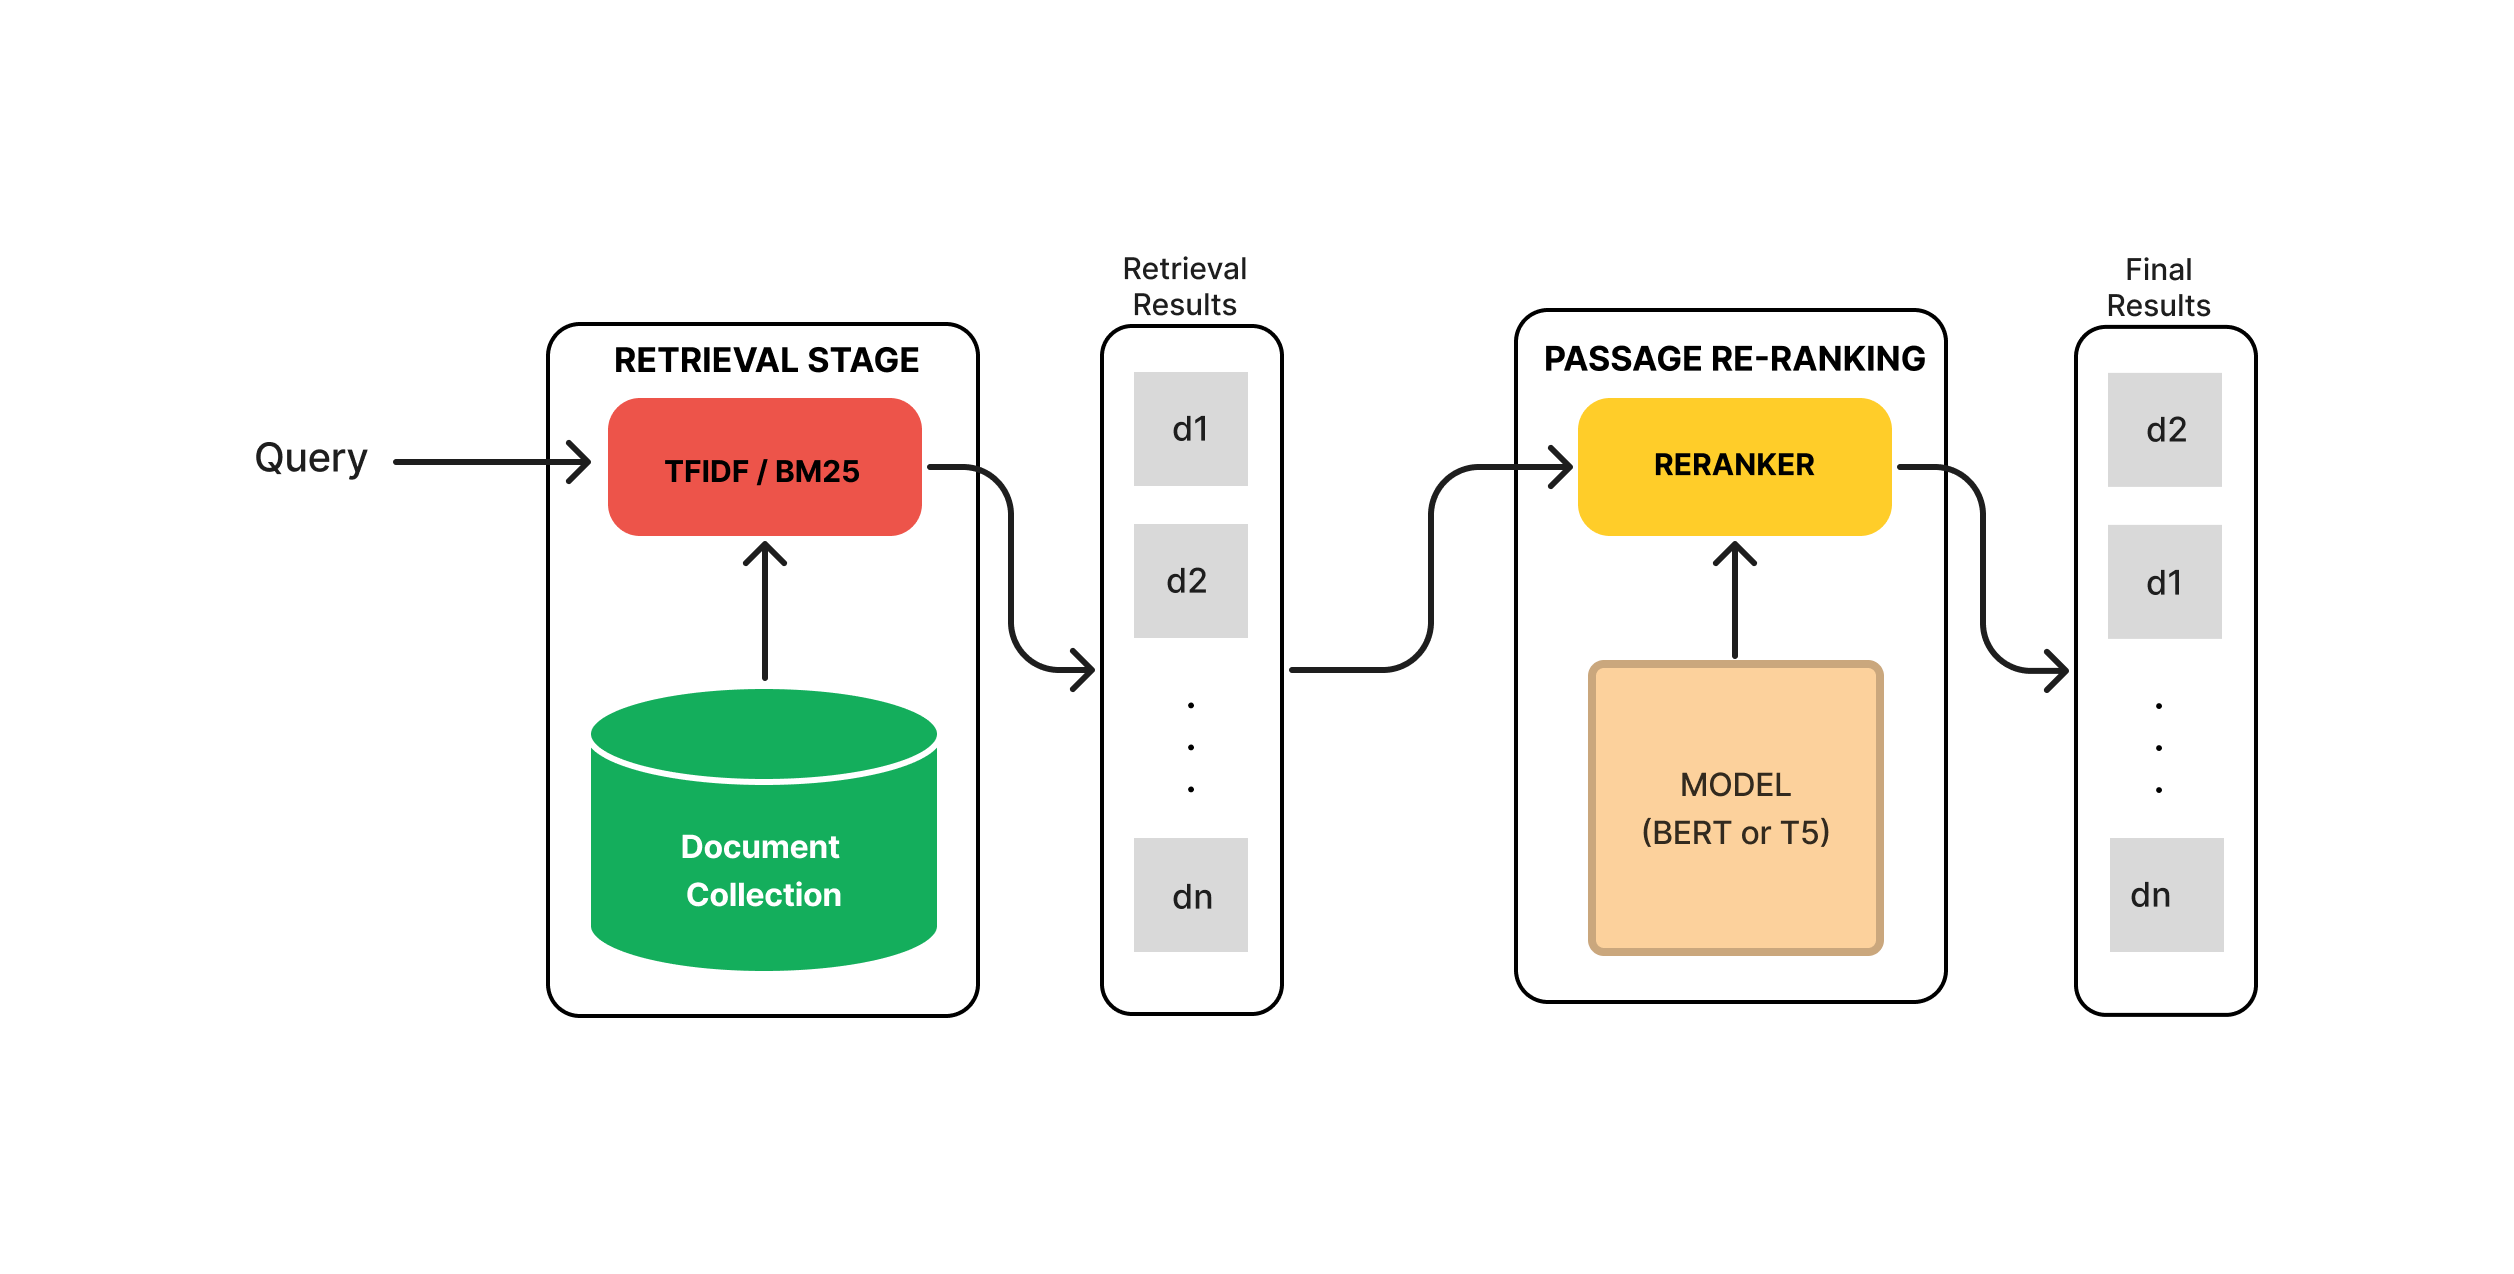
\includegraphics[width=0.8\linewidth]{figure/rerank_framework.png}
  \caption{Retrieve-than-rerank framework}
  \label{fig:rerank}
\end{figure}
We achieved this by leveraging a library called PyGaggle\cite{pygaggle}, which provides some deep neural architectures for text ranking and question answering, and two transformer-based models, T5 and BERT, with different checkpoints and even our own trained checkpoint using code from another library\cite{gao2021lce}. \\

In our system, we can choose how many documents are to be reranked from the top for two reasons: the first is raw computing performance, reranking all 1000 retrieved documents takes a long time and we don't have machines powerful enough to handle it; the second is that we saw that reranking more than 50 documents drops our measures down, even below the baseline measure without reranking.\\
Our first approach to reranking was to consider only the scores returned by the models to rerank the documents but we then switched to an approach where we consider also the BM25 score as follows. Let $Score_{BM25}(i)$ the score given by BM25 for the document at rank $i$ and $Score_{rr}(i)$ the score given by the reranker for the document at rank $i$, and let $n$ be the total number of reranked documents, we define: 
\begin{equation}
nScore_{rr}(i) = \bigg(Score_{rr}(i)+\min_{j\in [1,n]}Score(j)\bigg)\cdot \frac{Score_{BM25}(1)}{Score_{rr}(1)}
\end{equation}
as the normalized score for the reranked documents, since the models returned a score in the range $[-10,+10]$, which was not suitable for our case.\\
In our first approach, we simply passed the score to Lucene's \texttt{ScoreDoc} object and we were done. But in this way, we would lose information about the ranking given by BM25, which is still relevant, so we defined a new score: 
\begin{equation}
finalScore(i) = mntr + (1-\alpha)\cdot Score_{BM25}(i)+\alpha\cdot nScore_{rr}(i)
\end{equation}
where $mntr$ is the maximum score from docs which are not reranked, in this way, we preserve the order of this docs. With this approach, we can give a weight to the reranker to find the balance and we do not lose the information given to us by the first stage. Note that $\alpha=1$ corresponds to considering only scores from the reranker. \\

\noindent \textbf{Pretrained Models}

We tried two transformer-based models, T5 and BERT since they are supported by PyGaggle. First, we tried T5\cite{RaffelShazeerRobertsLeeNarangMatenaZhouLiLiuT5}, but with BERT\cite{devlin2019bert} we got better results. Starting from the same base model, t5-base\cite{t5base} for T5 bert-base-uncased\cite{bertbase} for BERT, we tried different checkpoints\footnote{saving the model's parameters and optimizer state during the training process} fine-tuned specifically for reranking tasks and we even tried to train our checkpoint. The pre-trained checkpoints that we used are: 
\begin{itemize}
\item \textit{monot5-base-msmarco-10k}\cite{castorinimonot5}
\item \textit{bert-base-mdoc-bm25}\cite{bertbasebm25}
\end{itemize}
The results for the T5 model are reported in Table~\ref{tab:t5-msmarco} and the results for the BERT model are reported in Table~\ref{tab:bert-mdoc}.
\begin{table}[!h]
\caption{\label{tab:t5-msmarco} monot5-base-msmarco-10k model with different number of documents to rerank}
\begin{tabular}{|l|l|l|}
\toprule
             & \textbf{nDCG} & \textbf{map} \\ 
\midrule
\textbf{0}   & 0,4075        & 0,2411       \\ 
\textbf{10}  & \textbf{0,414}         & \textbf{0,2502}       \\ 
\textbf{20}  & 0,4119        & 0,2477       \\ 
\textbf{50}  & 0,4083        & 0,242        \\ 
\textbf{100} & 0,405         & 0,2376       \\ 
\textbf{250} & 0,3987        & 0,2301\\
\bottomrule
\end{tabular}
\end{table}

\begin{table}[!h]
\caption{\label{tab:bert-mdoc}bert-base-mdoc-bm25 model with different number of documents to rerank}
\begin{tabular}{|l|l|l|}
\toprule
             & \textbf{nDCG} & \textbf{map} \\ 
\midrule
\textbf{0}   & 0,4075        & 0,2411       \\ 
\textbf{10}  & 0,4207         & 0,2608       \\ 
\textbf{20}  & \textbf{0,4222}        & \textbf{0,2617}       \\ 
\textbf{50}  & 0,4212        & 0,2598        \\ 
\textbf{100} & 0,4184         & 0,2563       \\ 
\textbf{250} & 0,4104        & 0,2478      \\
\bottomrule
\end{tabular}
\end{table}
The BERT pretrained checkpoint with 20 reranked documents improved \ac{nDCG} by $3.56\%$ and \ac{MAP} by $8.5\%$.\\

\noindent \textbf{Training our own checkpoint}\\
At this point, BERT gave us good results so we took it a step further and we tried to find ways to finetune it to our data. The training process is pretty straightforward: 
\begin{itemize}
\item \textbf{Data pre-processing}. Transformers expect batches of tensors as input, so we need to preprocess our data to the expected format. For processing textual data the tokenizer tool is used, which splits text into tokens; in our case, we exploit the pre-trained BERT tokenizer which returns tokens that are not necessarily words, but rather subwords: frequently used words are (or should) not split into smaller subwords, but rare words should be decomposed into meaningful subwords \cite{HfTokenizer}. Further, the tokenizer adds, at the beginning and at the end, two special tokens, respectively \texttt{[CLS]} and \texttt{[SEP]}. The tokenizer returns a dictionary with three items: 
	\begin{itemize}
		\item \texttt{input\_ids}, indices corresponding to each token in the sentence
		\item \texttt{attention\_mask}, indicates whether a token should be attended to or not
		\item \texttt{token\_type\_ids}, identifies which sequence a token belongs to when there is more than one sequence
	\end{itemize}
An important note is that BERT accepts input sequences of up to 512 tokens, so the tokenizer truncates longer documents. 
\item \textbf{Training}. The easiest way to train is to use the Trainer API from PyTorch \cite{HfTrainer}.
\end{itemize} 
To ease development, we used a package for training deep language model rerankers\cite{gao2021lce} and adapted the example code to our collection. The trainer in the package expects the training data in a JSON file with the format shown in Listing~\ref{lst:train-format}. 

\begin{lstlisting}[label={lst:train-format},caption={Train format},captionpos=b, xleftmargin=.2\textwidth]
{
    "qry": {
        "qid": str,
        "query": List[int],
    },
    "pos": List[
        {
            "pid": str,
            "passage": List[int],
        }
    ],
    "neg": List[
        {
            "pid": str,
            "passage": List[int]
        }
    ]
}
\end{lstlisting}

The \texttt{convert\_to\_training.py} takes care of converting data to the training file, given the ranking file, the qrels, the query collection and the docs collection. Then it is sufficient to use the \texttt{trainer.py} code to get the trained model. Unfortunately, we don't have access to sufficiently powerful machines so we were forced to train on a Google Colab notebook. This came with a major drawback: the maximum runtime is 12 hours, so we couldn't train on more than 1 epoch since a 2 epoch model was estimated to take 15 hours to train. This obviously tanked our model performances, and, as we can see in Table~\ref{tab:own-model}.

\begin{table}[!h]
\caption{\label{tab:own-model}Our trained model with different number of documents to rerank}
\begin{tabular}{|l|l|l|}
\toprule
             & \textbf{nDCG} & \textbf{map} \\
\midrule
\textbf{0}   & 0,4075        & 0,2411       \\ 
\textbf{10}  & 0,3910         & 0,2253       \\ 
\textbf{20}  & 0,3741       & 0,1975       \\ 
\textbf{50}  & 0,3405        & 0,1580        \\ 
\bottomrule
\end{tabular}
\end{table}

\noindent The Colab notebook with all the hyperparameters can be found at \url{https://colab.research.google.com/drive/1oFeYSkR31A-MUibwWrfNcKLUyPxEYbOq?usp=sharing}. \\
The trained model can be found at \url{https://huggingface.co/enricobolzonello/clef_longeval}.\\

\noindent \textbf{Integrating with Lucene}\\
One problem that emerged while working with the reranker was integrating it with Lucene since the reranker is written in Python and our main program is in Java. To solve the issue we came up with three approaches: 
\begin{enumerate}
\item passing intermediate text files, with documents, query to the reranker and returning the ranking to Java. This solution was used for initial testing but was deemed too inefficient and prone to errors
\item using Python as the system's entry point and using the PyJNIus library\cite{pyjnius} to access Java classes. The same approach was used by Birch \cite{Birch}, but we should have changed the classes too much to integrate tightly the reranker and more importantly we didn't want to change the entry point of our system 
\item our final solution was to call in some way Python from Java
\end{enumerate}
The library we used to achieve this is JEP \cite{jep}, which uses \ac{JNI} and the CPython API to start up the Python interpreter inside the \ac{JVM}. Thanks to the Python interpreter, we can call, at each query, the reranker which returns a list of generic \texttt{Object}s that is converted to a list of \texttt{Float}.

\section{Experimental Setup}
\label{sec:setup}

The experimental setup of this project consists of the following:
\begin{itemize}
    \item The \emph{project} is available at \url{https://bitbucket.org/upd-dei-stud-prj/seupd2223-faderic/src/master/};
    \item The \emph{collections} are taken from \url{https://clef-longeval.github.io/data/};
    \item The \emph{evaluation tool} used is trec\_eval v9.0.7, available \url{https://trec.nist.gov/trec_eval/};
    \item To compute the runs we have used the following \emph{hardware}: CPU AMD Ryzen 7 2700, GPU Zotac GeForce RTX 2060 6 GB, RAM 16 GB DDR4;
\end{itemize}

In order to reproduce the runs for this system, it is necessary to follow the instructions given in the project's ReadMe file.

\section{Results}
\label{sec:results}

In this Section we will show and analyze the results obtained by our system.
In particular, Section~\ref{subsec:train-res} will be about the results of all the runs produced by our system on the training collection during its development, while Section~\ref{subsec:test-res} will consist of a statistical analysis of the runs submitted to \ac{CLEF} on the test collections.

\subsection{Training results}
\label{subsec:train-res}

We have \emph{combined} the different components explained in Section~\ref{sec:methodology} and we conducted a thorough experimentation process to identify the best-performing system for our task. 
By tuning the parameters of each component and selecting the optimal ones, we were able to build a 
system that addresses the persistence issue of \ac{IR} systems.
In Table~\ref{tab:map-ndcg-table} are reported the \ac{MAP} and \ac{nDCG} scores obtained on those systems.

\begin{table}[tbp]
\caption{\ac{nDCG} and \ac{MAP} values on train collection}
  \label{tab:map-ndcg-table}
    \centering
    \begin{tabular}{|p{0.7\linewidth}|p{0.075\linewidth}|p{0.075\linewidth}|}
	\toprule
	\textbf{Run name} & \textbf{nDCG} & \textbf{MAP} \\
	\midrule
        \raggedright FADERIC\_French-BM25-Stop50-LightStem-Shingle-Fuzzy-SynCustom-Rerank20W6 & 0.4274 & 0.2671 \\ 
        FADERIC\_French-BM25-Stop50-LightStem-Shingle-Fuzzy-Rerank30 & 0.4230 & 0.2632 \\ 
        FADERIC\_French-BM25-Stop50-LightStem-Shingle-Fuzzy-SynCustom & 0.4079 & 0.2416 \\ 
        FADERIC\_French-BM25Tuned-Stop50-LightStem-Shingle-Fuzzy & 0.4047 & 0.2383 \\ 
        FADERIC\_French-BM25-StopDefault-SnowStem & 0.3786 & 0.2110 \\ 
        FADERIC\_English-BM25-Stop50-KStem-Shingle-Fuzzy-SynPOS\\-Rerank30 & 0.3271 & 0.1877 \\ 
        FADERIC\_English-BM25-Stop50-KStem-Shingle-Fuzzy-Rerank30 & 0.3527 & 0.1873 \\ 
        FADERIC\_French-BM25-Stop50-LightStem-Shingle-Fuzzy\\-TrainedRerank30 & 0.3599 & 0.1799 \\ 
        FADERIC\_French-LMDirichlet-Stop50-LightStem & 0.3398 & 0.1731 \\ 
        FADERIC\_English-BM25-Stop50-KStem-Shingle-Fuzzy-SynPOS & 0.3081 & 0.1634 \\ 
        FADERIC\_English-BM25-StopDefault-SnowStem & 0.2927 & 0.1490 \\ 
        FADERIC\_English-LMDirichlet-Stop50-KStem & 0.2612 & 0.1228 \\ 
	\bottomrule
    \end{tabular}
\end{table}

The keywords reported in the names of the runs have the following meanings:
\begin{itemize}
	\item French: used documents and queries from the French collection
	\item English: used documents and queries from the English collection
	\item BM25: used Okapi BM25 similarity (with default parameters)
	\item BM25Tuned: used Okapi BM25 similarity, with parameters tuned on training collection: k1=1.6 and b=0.7
	\item LMDirichlet: used Dirichlet smoothing (with default parameter)
	\item StopDefault: used Lucene's default stop words list
	\item Stop50: used stoplist built by picking the 50 most frequent terms in the documents indexed without stoplist and stemming
	\item LightStem: used the Light stemmer
	\item KStem: used Krovetz stemmer
	\item SnowStem: the Snowball stemmer
	\item Shingle: used word N-grams (max window size = 3) query expansion
	\item Fuzzy: used fuzzyness (threshold parameter = 10) query expansion
	\item SynCustom: used custom synonyms list
	\item SynPOS: used WordNet synonym list together with OpenNLP \ac{PoS} tagging
	\item Rererank20W6: used reranker, reranking 20 documents with weight 0.6 given to the reranker scores
	\item Rererank30: used reranker, reranking 30 documents with weight 1 given to the reranker scores
	\item TrainedRerank30: used reranker, reranking 30 documents using our custom model
\end{itemize}

During the tuning of our system, we primarily focused on \ac{MAP} and \ac{nDCG}. However, in order to perform a more \emph{comprehensive} analysis, 
we also considered additional measures such as Precision and Recall: the first one is the fraction of retrieved 
documents that are relevant to the user's query, indicating a measure of the accuracy of the system,
while with the second is a measure of the completeness of the system in retrieving all relevant results, 
computed by the fraction of relevant documents retrieved.

In Figure~\ref{fig:precision-recall-curve}, we show the \emph{interpolated} Precision-Recall curve, which can be useful to show the inverse relationship between Precision and Recall, indicating the \emph{trade-off} between these two measures.

\begin{figure}[tbp]
  \centering
  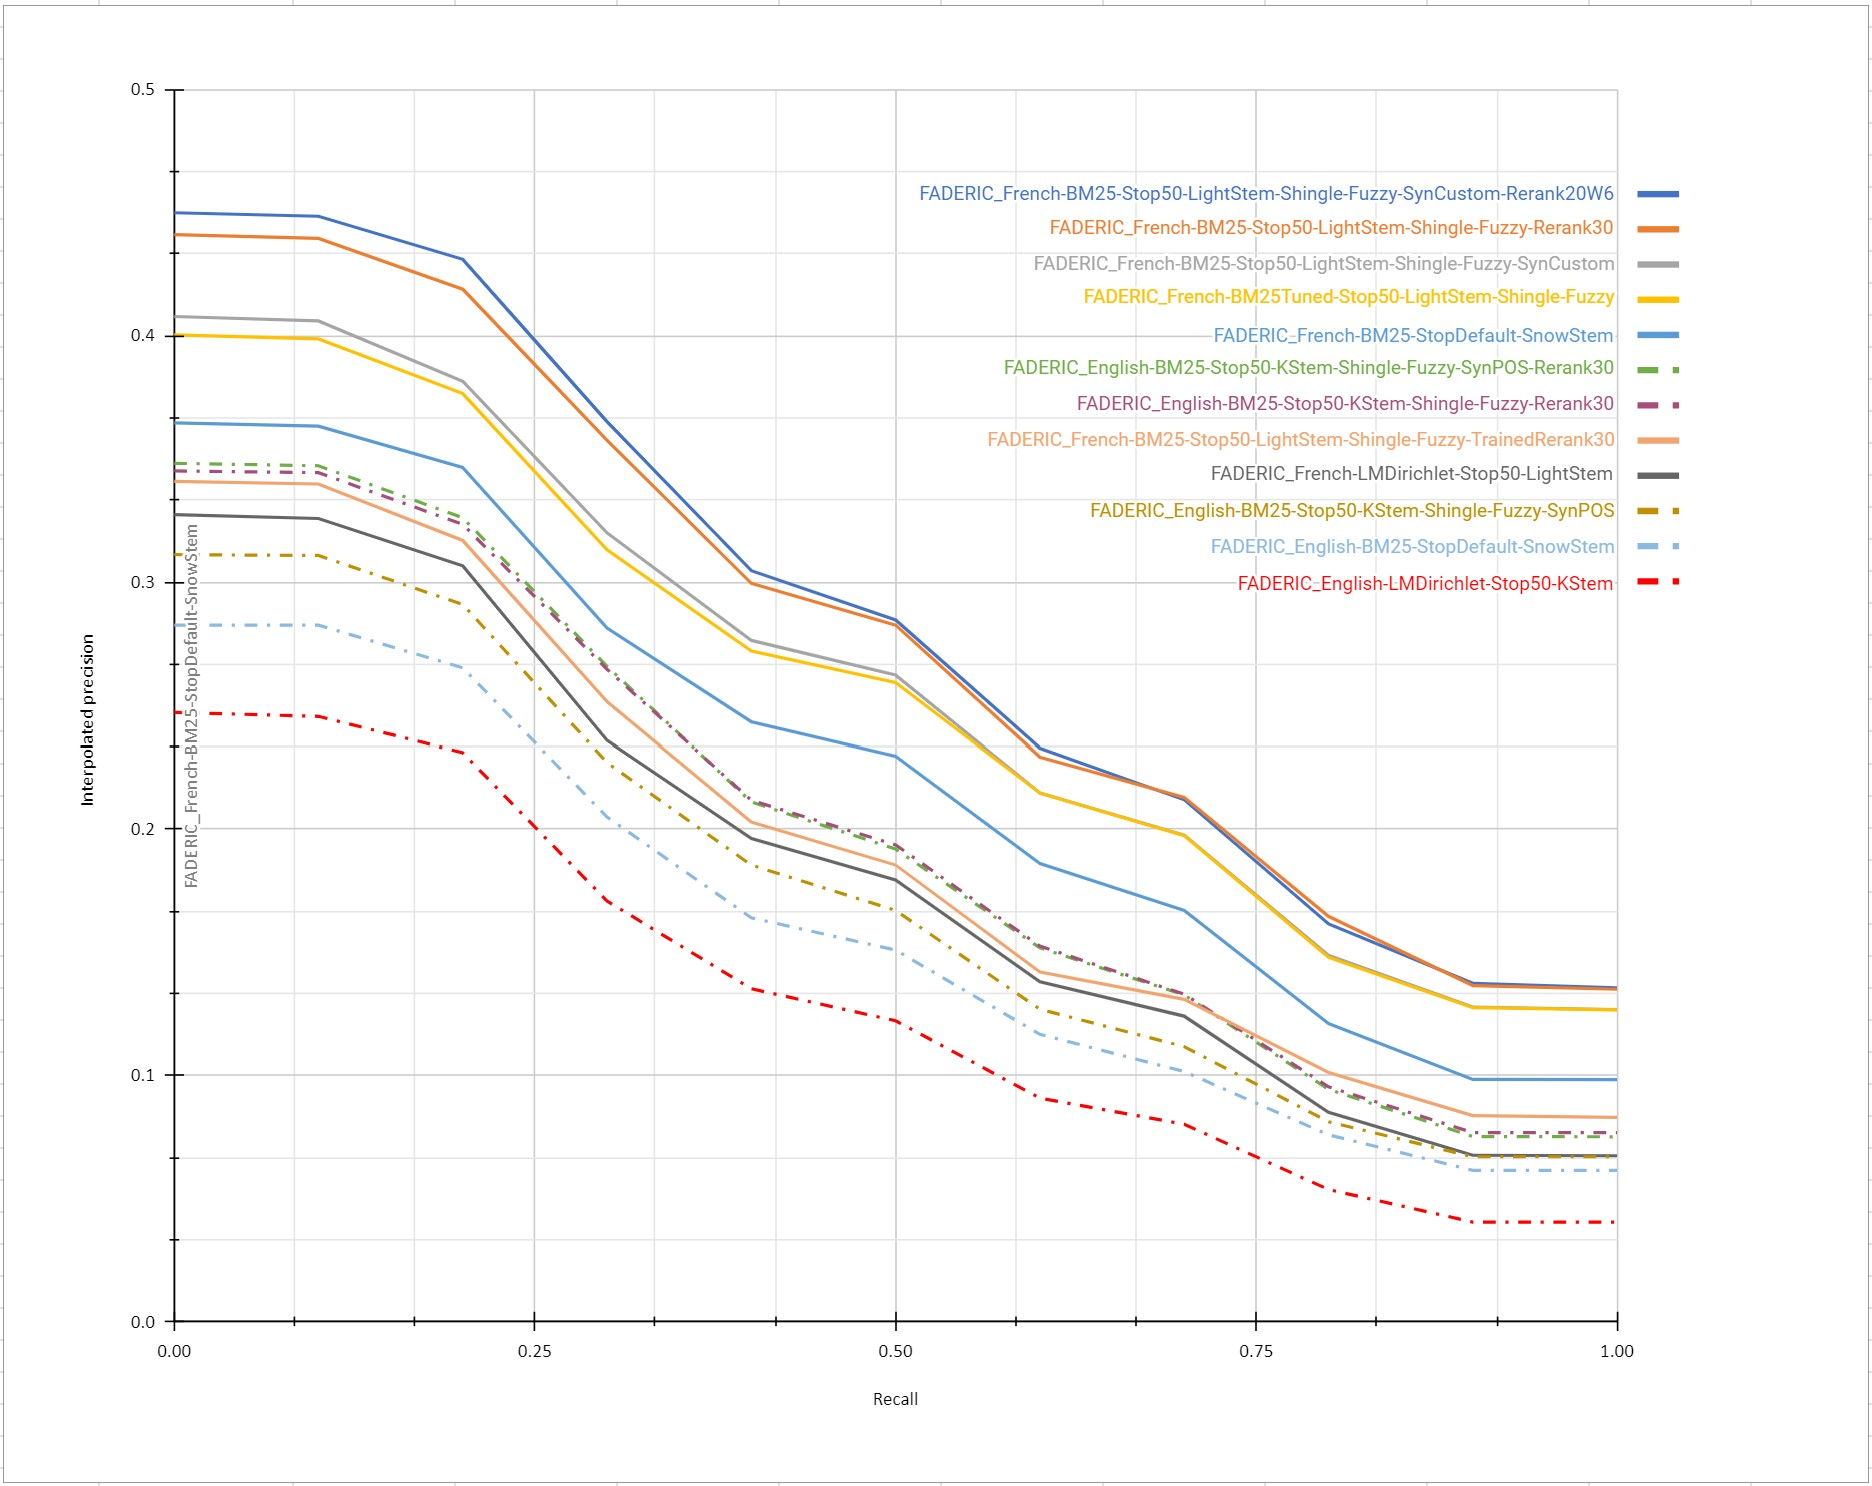
\includegraphics[width=1\linewidth]{figure/prec-recall.jpg}
  \caption{Interpolated Precision-Recall curve on train collection}
  \label{fig:precision-recall-curve}
\end{figure}

\pagebreak

In Table~\ref{tab:all-measures-french} and in Table~\ref{tab:all-measures-english} we have reported a more complete list of scores respectively for the French and English runs. For space reasons, we label the runs as: 

\begin{itemize}
	\item fr\_1 = FADERIC\_French-BM25-Stop50-LightStem-Shingle-Fuzzy-SynCustom\\-Rerank20W6
	\item fr\_2 = FADERIC\_French-BM25-Stop50-LightStem-Shingle-Fuzzy-Rerank30
	\item fr\_3 = FADERIC\_French-BM25-Stop50-LightStem-Shingle-Fuzzy-SynCustom
	\item fr\_4 = FADERIC\_French-BM25Tuned-Stop50-LightStem-Shingle-Fuzzy
	\item fr\_5 = FADERIC\_French-BM25-StopDefault-SnowStem
	\item fr\_6 = FADERIC\_French-BM25-Stop50-LightStem-Shingle-Fuzzy-TrainedRerank30
	\item fr\_7 = FADERIC\_French-LMDirichlet-Stop50-LightStem
	\item en\_1 = FADERIC\_English-BM25-Stop50-KStem-Shingle-Fuzzy-SynPOS-Rerank30
	\item en\_2 = FADERIC\_English-BM25-Stop50-KStem-Shingle-Fuzzy-Rerank30
	\item en\_3 = FADERIC\_English-BM25-Stop50-KStem-Shingle-Fuzzy-SynPOS
	\item en\_4 = FADERIC\_English-BM25-StopDefault-SnowStem
	\item en\_5 =FADERIC\_English-LMDirichlet-Stop50-KStem
\end{itemize}

\begin{table}[tbp]
\caption{Measures for French runs on train collection}
  \label{tab:all-measures-french}
    \centering
    \begin{tabular}{|l|l|l|l|l|l|l|l|l|l|}
    	\toprule
        runid & all & fr\_1 & fr\_2 & fr\_3 & fr\_4 & fr\_5 & fr\_6 & fr\_7  \\
	\midrule
        num\_q & all & 672 & 672 & 672 & 672 & 672 & 672 & 672  \\ 
        num\_ret & all & 660838 & 660838 & 660838 & 660838 & 658471 & 660838 & 658512  \\ 
        num\_rel & all & 2626 & 2626 & 2626 & 2626 & 2626 & 2626 & 2626  \\ 
        num\_rel\_ret & all & 2316 & 2318 & 2316 & 2323 & 2271 & 2318 & 2156  \\ \midrule
	ndcg & all & \textbf{0.4274} & 0.4230 & 0.4079 & 0.4047 & 0.3786 & 0.3599 & 0.3398  \\ \midrule
        map & all & \textbf{0.2670} & 0.2632 & 0.2416 & 0.2383 & 0.2110 & 0.1799 & 0.1731  \\ 
        gm\_map & all & \textbf{0.0786} & 0.0765 & 0.0702 & 0.0696 & 0.0545 & 0.0552 & 0.0394  \\ \midrule
        Rprec & all & \textbf{0.2280} & 0.2278 & 0.1987 & 0.1946 & 0.1747 & 0.1365 & 0.1469  \\ 
        bpref & all & \textbf{0.4128} & 0.4122 & 0.4085 & 0.4063 & 0.3753 & 0.3701 & 0.3561  \\ 
        recip\_rank & all & 0.4222 & 0.4140 & 0.3824 & 0.3734 & 0.3424 & 0.3170 & 0.3134  \\ \midrule
        iprec\_at\_recall\_0.00 & all & \textbf{0.4499} & 0.4410 & 0.4078 & 0.4003 & 0.3646 & 0.3409 & 0.3274  \\ 
        iprec\_at\_recall\_0.10 & all & \textbf{0.4485} & 0.4395 & 0.4060 & 0.3987 & 0.3633 & 0.3398 & 0.3258  \\ 
        iprec\_at\_recall\_0.20 & all & \textbf{0.4310} & 0.4189 & 0.3815 & 0.3765 & 0.3465 & 0.3169 & 0.3066  \\ 
        iprec\_at\_recall\_0.30 & all & \textbf{0.3651} & 0.3575 & 0.3200 & 0.3131 & 0.2813 & 0.2515 & 0.2359  \\ 
        iprec\_at\_recall\_0.40 & all & \textbf{0.3046} & 0.2995 & 0.2763 & 0.2720 & 0.2433 & 0.2030 & 0.1963  \\ 
        iprec\_at\_recall\_0.50 & all & \textbf{0.2846} & 0.2825 & 0.2623 & 0.2592 & 0.2296 & 0.1855 & 0.1795  \\ 
        iprec\_at\_recall\_0.60 & all & \textbf{0.2328} & 0.2293 & 0.2147 & 0.2147 & 0.1861 & 0.1421 & 0.1381  \\ 
        iprec\_at\_recall\_0.70 & all & 0.2120 & \textbf{0.2130} & 0.1976 & 0.1974 & 0.1671 & 0.1310 & 0.1242  \\ 
        iprec\_at\_recall\_0.80 & all & 0.1616 & \textbf{0.1647} & 0.1489 & 0.1481 & 0.1212 & 0.1013 & 0.0851  \\ 
        iprec\_at\_recall\_0.90 & all & \textbf{0.1375} & 0.1366 & 0.1279 & 0.1276 & 0.0985 & 0.0838 & 0.0677  \\ 
        iprec\_at\_recall\_1.00 & all & \textbf{0.1357} & 0.1351 & 0.1268 & 0.1267 & 0.0984 & 0.0831 & 0.0675  \\ \midrule
        P\_5 & all & \textbf{0.2074} & 0.2065 & 0.1875 & 0.1827 & 0.1637 & 0.1315 & 0.1375  \\ 
        P\_10 & all & \textbf{0.1603} & 0.1560 & 0.1472 & 0.1469 & 0.1332 & 0.1007 & 0.1088  \\ 
        P\_15 & all & 0.1233 & \textbf{0.1243} & 0.1183 & 0.1167 & 0.1090 & 0.0869 & 0.0889  \\ 
        P\_20 & all & 0.0990 & \textbf{0.1022} & 0.0990 & 0.0990 & 0.0901 & 0.0799 & 0.0753  \\ 
        P\_30 & all & \textbf{0.0748} & 0.0743 & \textbf{0.0748} & 0.0743 & 0.0683 & 0.0742 & 0.0580  \\ 
        P\_100 & all & 0.0279 & 0.0279 & 0.0279 & \textbf{0.0280} & 0.0267 & 0.0279 & 0.0232  \\ 
        P\_200 & all & 0.0150 & 0.0150 & 0.0150 & \textbf{0.0151} & 0.0146 & 0.0150 & 0.0133  \\ 
        P\_500 & all & \textbf{0.0065} & \textbf{0.0065} & \textbf{0.0065} & \textbf{0.0065} & 0.0064 & \textbf{0.0065} & 0.0060  \\ 
        P\_1000 & all & 0.0034 & 0.0034 & 0.0034 & \textbf{0.0035} & 0.0034 & 0.0034 & 0.0032  \\ \midrule
        recall\_5 & all & \textbf{0.2738} & 0.2732 & 0.2478 & 0.2417 & 0.2106 & 0.1749 & 0.1802  \\ 
        recall\_10 & all & \textbf{0.4167} & 0.4042 & 0.3830 & 0.3828 & 0.3402 & 0.2606 & 0.2789  \\ 
        recall\_15 & all & 0.4724 & \textbf{0.4757} & 0.4560 & 0.4499 & 0.4203 & 0.3366 & 0.3380  \\ 
        recall\_20 & all & 0.5034 & \textbf{0.5193} & 0.5032 & 0.5051 & 0.4595 & 0.4119 & 0.3814  \\ 
        recall\_30 & all & \textbf{0.5710} & 0.5657 & \textbf{0.5710} & 0.5677 & 0.5187 & 0.5651 & 0.4412  \\ 
        recall\_100 & all & 0.7022 & 0.7019 & 0.7022 & \textbf{0.7028} & 0.6688 & 0.7019 & 0.5816  \\ 
        recall\_200 & all & 0.7555 & 0.7560 & 0.7555 & \textbf{0.7587} & 0.7283 & 0.7560 & 0.6729  \\ 
        recall\_500 & all & 0.8219 & 0.8232 & 0.8219 & \textbf{0.8235} & 0.7994 & 0.8232 & 0.7574  \\ 
        recall\_1000 & all & 0.8663 & 0.8662 & 0.8663 & \textbf{0.8685} & 0.8485 & 0.8662 & 0.8072  \\
	\bottomrule
    \end{tabular}
\end{table}

\begin{table}[tbp]
\caption{Measures for English runs on train collection}
  \label{tab:all-measures-english}
    \centering
    \begin{tabular}{|l|l|l|l|l|l|l|}
    \toprule
	runid & all & en\_1 & en\_2 & en\_3 & en\_4 & en\_5  \\
	\midrule
        num\_q & all & 672 & 672 & 672 & 671 & 671  \\ 
        num\_ret & all & 655602 & 655602 & 655602 & 654919 & 654764  \\ 
        num\_rel & all & 2626 & 2626 & 2626 & 2623 & 2623  \\ 
        num\_rel\_ret & all & 1924 & 1915 & 1924 & 1878 & 1765  \\ \midrule
	ndcg & all & \textbf{0.3271} & 0.3257 & 0.3081 & 0.2927 & 0.2612  \\ \midrule
        map & all & \textbf{0.1877} & 0.1873 & 0.1634 & 0.1490 & 0.1228  \\ 
        gm\_map & all & \textbf{0.0221} & 0.0215 & 0.0195 & 0.0164 & 0.0122  \\ \midrule
        Rprec & all & 0.1706 & \textbf{0.1708} & 0.1385 & 0.1253 & 0.1092  \\ 
        bpref & all & \textbf{0.3536} & 0.3524 & 0.3417 & 0.3263 & 0.3139  \\ 
        recip\_rank & all & \textbf{0.3322} & 0.3289 & 0.2967 & 0.2697 & 0.2364  \\ \midrule
        iprec\_at\_recall\_0.00 & all & \textbf{0.3482} & 0.3451 & 0.3111 & 0.2825 & 0.2471  \\ 
        iprec\_at\_recall\_0.10 & all & \textbf{0.3472} & 0.3444 & 0.3108 & 0.2825 & 0.2455  \\ 
        iprec\_at\_recall\_0.20 & all & \textbf{0.3261} & 0.3234 & 0.2909 & 0.2652 & 0.2310  \\ 
        iprec\_at\_recall\_0.30 & all & \textbf{0.2658} & 0.2646 & 0.2270 & 0.2050 & 0.1709  \\ 
        iprec\_at\_recall\_0.40 & all & 0.2111 & \textbf{0.2118} & 0.1855 & 0.1641 & 0.1353  \\ 
        iprec\_at\_recall\_0.50 & all & 0.1920 & \textbf{0.1937} & 0.1671 & 0.1510 & 0.1223  \\ 
        iprec\_at\_recall\_0.60 & all & 0.1519 & \textbf{0.1526} & 0.1270 & 0.1168 & 0.0909  \\ 
        iprec\_at\_recall\_0.70 & all & 0.1328 & \textbf{0.1331} & 0.1118 & 0.1017 & 0.0803  \\ 
        iprec\_at\_recall\_0.80 & all & 0.0945 & \textbf{0.0955} & 0.0813 & 0.0760 & 0.0538  \\ 
        iprec\_at\_recall\_0.90 & all & 0.0753 & \textbf{0.0769} & 0.0671 & 0.0616 & 0.0406  \\ 
        iprec\_at\_recall\_1.00 & all & 0.0752 & \textbf{0.0769} & 0.0671 & 0.0616 & 0.0406  \\ \midrule
        P\_5 & all & \textbf{0.1542} & \textbf{0.1542} & 0.1345 & 0.1195 & 0.1019  \\ 
        P\_10 & all & \textbf{0.1137} & 0.1131 & 0.1042 & 0.0954 & 0.0793  \\ 
        P\_15 & all & \textbf{0.0904} & 0.0898 & 0.0835 & 0.0784 & 0.0650  \\ 
        P\_20 & all & \textbf{0.0745} & 0.0732 & 0.0705 & 0.0662 & 0.0543  \\ 
        P\_30 & all & 0.0536 & 0.053 & \textbf{0.0537} & 0.0513 & 0.0433  \\ 
        P\_100 & all & 0.0208 & \textbf{0.0209} & 0.0208 & 0.0201 & 0.0179  \\ 
        P\_200 & all & \textbf{0.0116} & 0.0115 & \textbf{0.0116} & 0.0113 & 0.0103  \\ 
        P\_500 & all &\textbf{ 0.0052} & \textbf{0.0052} & \textbf{0.0052} & 0.0051 & 0.0048  \\ 
        P\_1000 & all & \textbf{0.0029} & 0.0028 & \textbf{0.0029} & 0.0028 & 0.0026  \\ \midrule
        recall\_5 & all & \textbf{0.2020} & 0.2017 & 0.1710 & 0.1512 & 0.1329  \\ 
        recall\_10 & all & \textbf{0.2909} & 0.2887 & 0.2628 & 0.2437 & 0.1988  \\ 
        recall\_15 & all & \textbf{0.3430} & 0.3404 & 0.3155 & 0.2970 & 0.2432  \\ 
        recall\_20 & all & \textbf{0.3745} & 0.3683 & 0.3523 & 0.3318 & 0.2727  \\ 
        recall\_30 & all & 0.4010 & 0.3970 & \textbf{0.4018} & 0.3861 & 0.3281  \\ 
        recall\_100 & all & 0.5140 & \textbf{0.5167} & 0.5151 & 0.500 & 0.4486  \\ 
        recall\_200 & all & 0.5769 & 0.5754 & \textbf{0.5774} & 0.5630 & 0.5180  \\ 
        recall\_500 & all & 0.6607 & 0.6597 & \textbf{0.6612} & 0.6443 & 0.6087  \\ 
        recall\_1000 & all & \textbf{0.7186} & 0.7150 & \textbf{0.7186} & 0.7027 & 0.6635  \\ 
        \bottomrule
    \end{tabular}
\end{table}

\pagebreak

Based on these results, we can derive the following considerations:

\begin{itemize}
	\item the runs on the French collections are significantly better than the ones on the English one, the reason for this is the \emph{automatic translation} of the document collection, which has led to errors and inconsistencies in the English one;
	\item the system performs better when configured to use BM25 similarity instead of the Dirichlet smoothing;
	\item the \emph{tuned} parameters on BM25 just gave slightly betters results, probably \emph{overfitting} the run we have tuned them on, for this reason we have chosen to use the default ones in most of the runs;
	\item the custom stoplist we have generated by picking the most frequent terms has outperformed Lucene's default ones because since it was based on the specific collection the \emph{effectiveness} of using a stoplist has been maximized;
	\item in both French and English the Snowball stemmer performed worse than the Light and Krovetz stemmer, respectively;
	\item the use of word N-grams improved the performances, allowing to have more \emph{contextual matches} by looking for group of words instead of single ones;
	\item synonyms have slightly improved the performances, this is due to the fact that sometimes they can be \emph{misleading} and retrieve documents that are not contextual with the query;
	\item the reranking is a very \emph{powerful} tool that has given a huge performance increase to our runs.
\end{itemize}

Based on the previous results and these considerations, we have decided to submit to \ac{CLEF} the following systems:
\begin{itemize}
	\item FADERIC\_French-BM25-Stop50-LightStem-Shingle-Fuzzy-SynCustom-Rerank20W6, i.e., the best system overall;
	\item FADERIC\_English-BM25-Stop50-KStem-Shingle-Fuzzy-SynPOS-Rerank30, i.e., the best system overall on the English collection;
	\item FADERIC\_French-BM25-Stop50-LightStem-Shingle-Fuzzy-SynCustom, i.e., the best system without the use of reranking;
	\item FADERIC\_French-BM25-Stop50-LightStem-Shingle-Fuzzy-Rerank30, i.e., the best system without the use of synonyms;
	\item FADERIC\_French-BM25Tuned-Stop50-LightStem-Shingle-Fuzzy, i.e., the best system without the use of both synonyms and reranking;

\end{itemize}


\subsection{Test results}
\label{subsec:test-res}

In this Section, we will analyze the performance of the submitted runs on heldout, short term and long term collections. At first, we will tackle the performance changes and then we will perform a \emph{statistical analysis}. In this last part, we will use ANOVA2 with a significance level $\alpha=0.05$ in order to find out if we can reject the \emph{null hypothesis}, i.e. there is no significant statistical difference between the results of the given runs. \\Then we will use Tukey's \ac{HSD} test to perform \emph{multiple} pairwise comparisons and determine which specific run means differ significantly from each other.

Since we have submitted four runs performed on the French collection and one on the English collection, in the statistical analysis we will compare to each other only the French runs.

\subsubsection{Heldout}
\label{subsubsec:heldout-res}

In Table~\ref{tab:heldout-map-ndcg-table} are reported the \ac{nDCG} and \ac{MAP} values obtained from the submitted runs on the heldout collection, while in Figure~\ref{fig:precision-recall-curve-heldout} is reported the interpolated Precision-Recall curve. Comparing these results with the ones obtained on training, shown in Table~\ref{tab:map-ndcg-table} and Figure~\ref{fig:precision-recall-curve} respectively, we can see that every run suffered a \emph{performance drop} over all the measures. This worsening was \emph{expected} and it can be due to the fact that the system has been tuned over a different set of queries. It should also be noticed that this set of queries is more than 6 times smaller compared to the training one, therefore the presence of some \emph{outliers} could have caused the mean performances to drop and to not be a good descriptor of the system.

Observing the \ac{nDCG} and \ac{AP} boxplots, shown in Figure~\ref{fig:heldout-boxplot}, we can notice that the runs performed on the French collection have a similar structure in terms of median values and interquartile ranges. We can also notice that, in the \ac{AP} boxplot, the reranked runs fr\_1, fr\_2 have longer whiskers, while the others show the presence of outliers.

From the ANOVA2 analysis, which results are reported in Table~\ref{tab:heldout-anova2}, we can see that $p\textrm{--}value>\alpha$, therefore we \emph{cannot reject} the null hypothesis. Moreover, from Tukey's \ac{HSD} multiple comparison shown in Figure~\ref{fig:heldout-hsd}, we can derive that the French runs can be considered to be similar to each other.

\begin{table}[tbp]
\caption{\ac{nDCG} and \ac{MAP} values on heldout collection}
  \label{tab:heldout-map-ndcg-table}
    \centering
    \begin{tabular}{|p{0.7\linewidth}|p{0.075\linewidth}|p{0.075\linewidth}|}
	\toprule
	\textbf{Run name} & \textbf{nDCG} & \textbf{MAP} \\
	\midrule
        FADERIC\_French-BM25-Stop50-LightStem-Shingle-Fuzzy-SynCustom-Rerank20W6 & 0.4169 & 0.2474 \\
        FADERIC\_French-BM25-Stop50-LightStem-Shingle-Fuzzy-Rerank30 & 0.4147 & 0.2416 \\
        FADERIC\_French-BM25-Stop50-LightStem-Shingle-Fuzzy-SynCustom & 0.4080 & 0.2376 \\
        FADERIC\_French-BM25Tuned-Stop50-LightStem-Shingle-Fuzzy & 0.4044 & 0.2324 \\
        FADERIC\_English-BM25-Stop50-KStem-Shingle-Fuzzy-SynPOS\\-Rerank30 & 0.3030 & 0.1626 \\
	\bottomrule
    \end{tabular}
\end{table}

\begin{figure}[tbp]
  \centering
  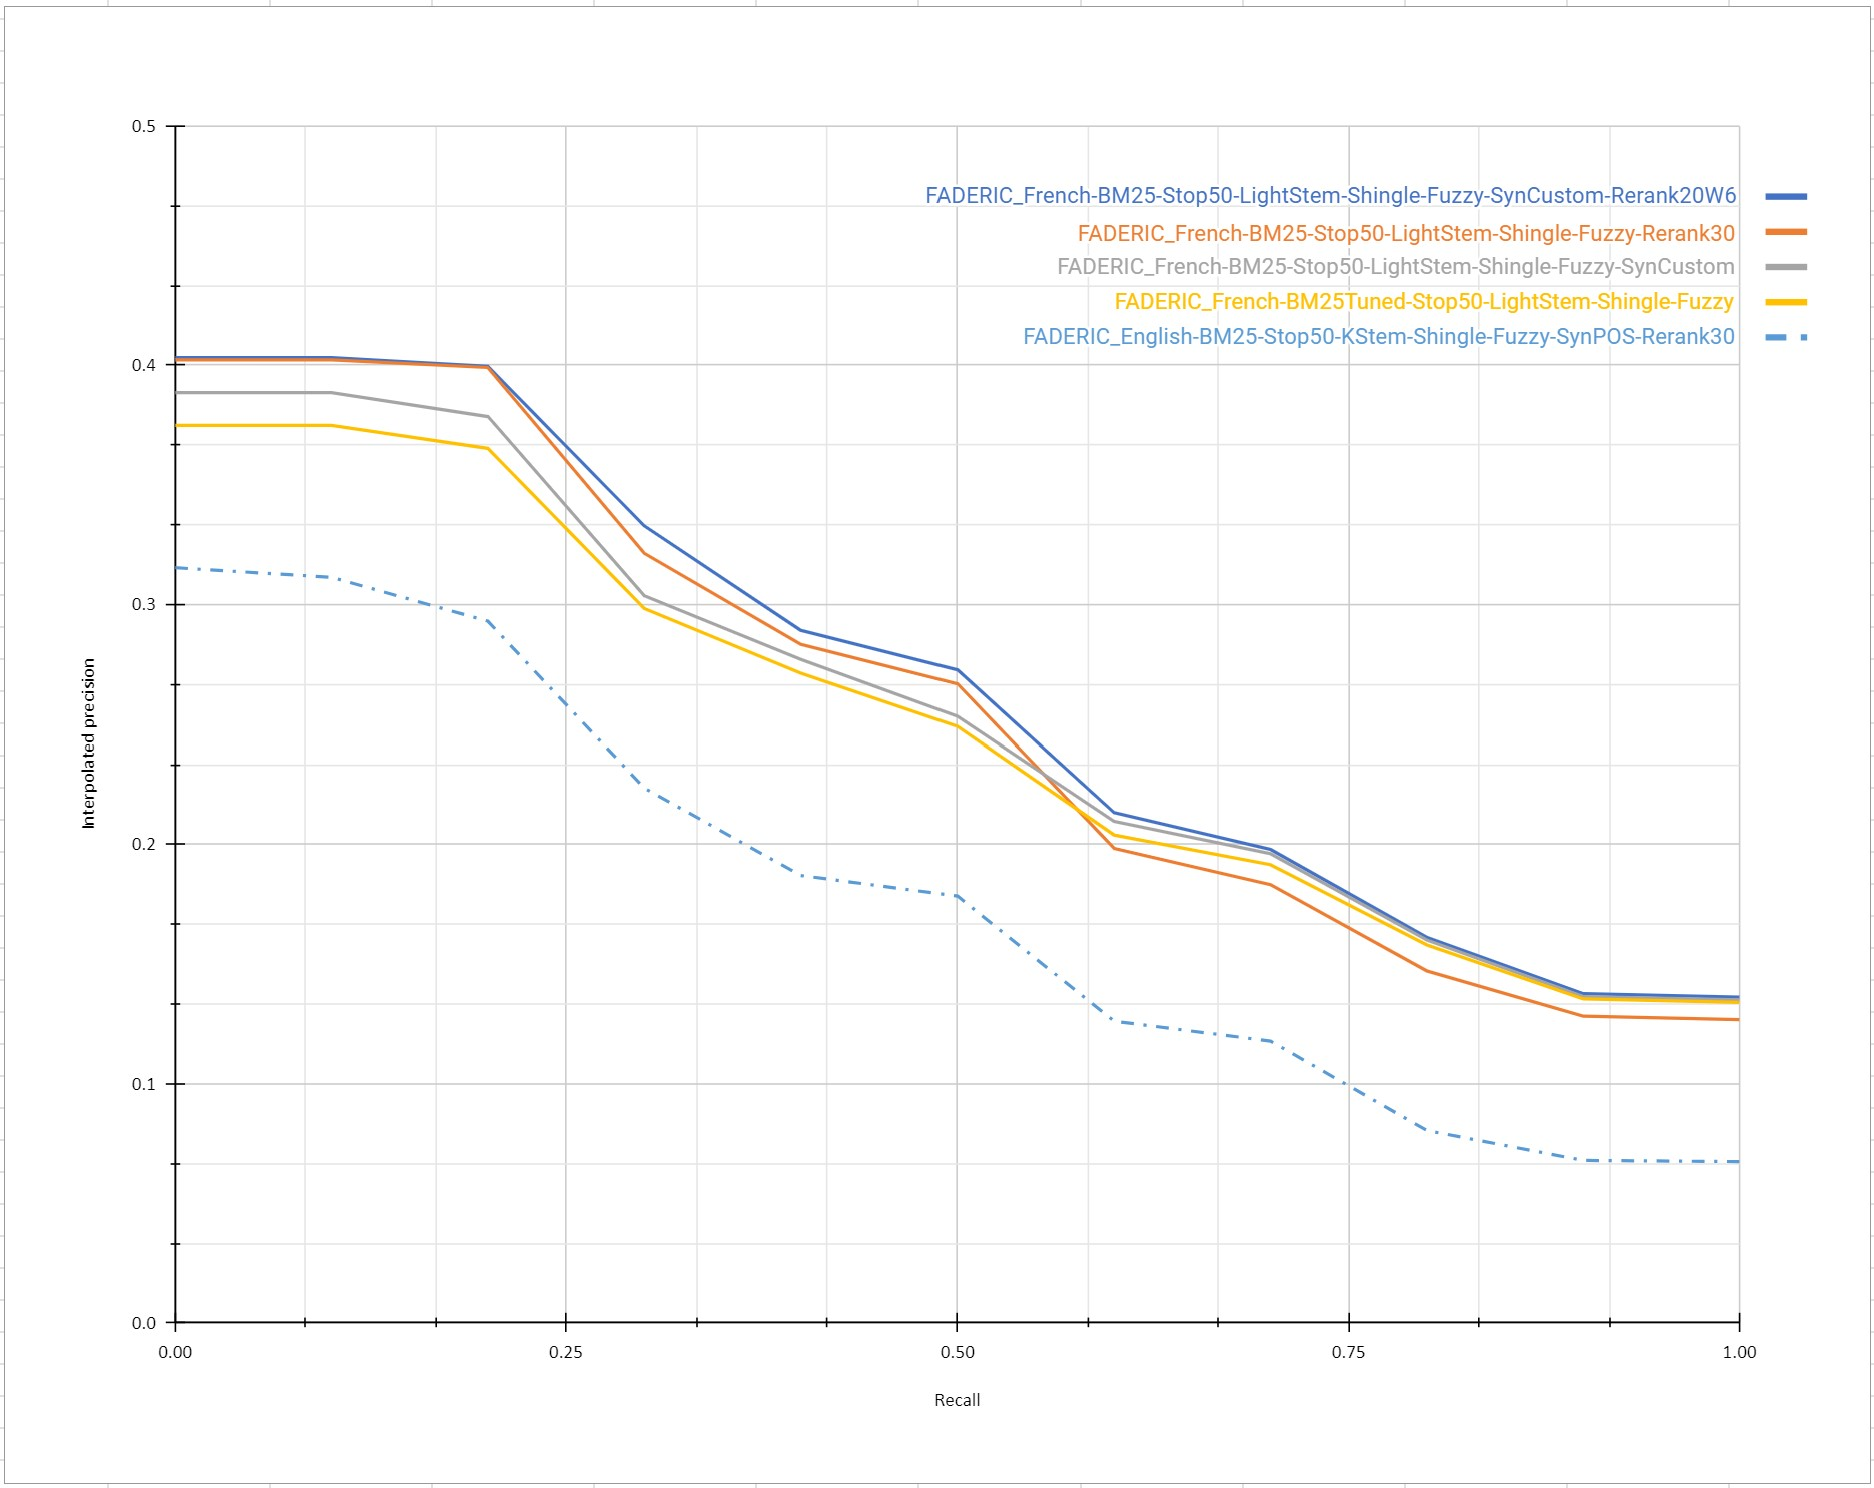
\includegraphics[width=1\linewidth]{figure/iprec-recall-HELDOUT.jpg}
  \caption{Interpolated Precision-Recall curve on heldout collection}
  \label{fig:precision-recall-curve-heldout}
\end{figure}

\begin{figure}[tbp]
     \centering
     \begin{subfigure}[b]{0.45\textwidth}
         \centering
         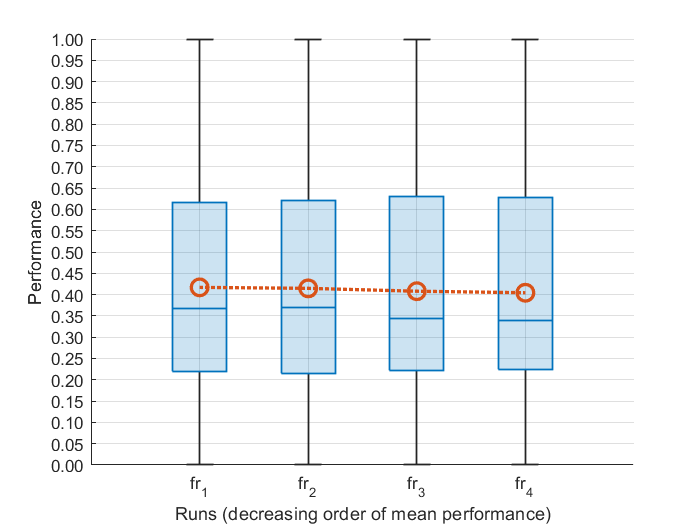
\includegraphics[width=\textwidth]{figure/heldout-ndcg-boxplot.png}
         \caption{\ac{nDCG}}
     \end{subfigure}
     \hfill
     \begin{subfigure}[b]{0.45\textwidth}
         \centering
         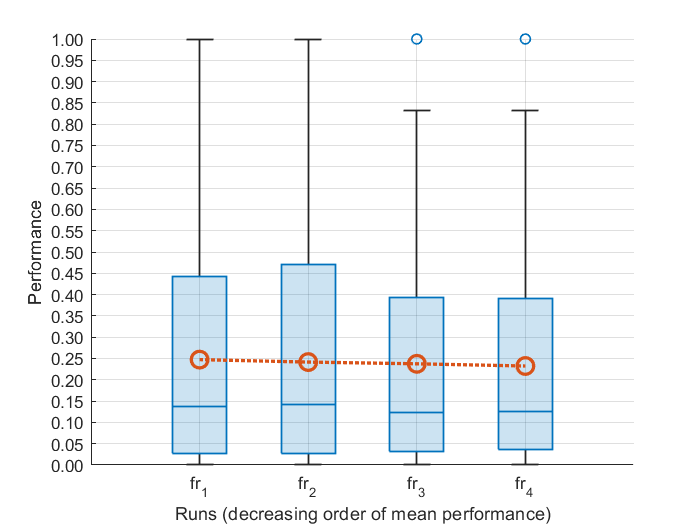
\includegraphics[width=\textwidth]{figure/heldout-map-boxplot.png}
         \caption{\ac{AP}}
     \end{subfigure}
        \caption{Box plot on heldout collection, the mean values are shown in red}
        \label{fig:heldout-boxplot}
\end{figure}

\begin{table}[tbp]
     \caption{ANOVA2 on heldout collection}
    \begin{subtable}[t]{1\textwidth}
        \centering
	\caption{\ac{nDCG}}
	\begin{tabular}{|l|l|l|l|l|l|}
	\toprule
        \textbf{Source} & \textbf{SS} & \textbf{df} & \textbf{MS} & \textbf{F} & \textbf{Prob$>$F} \\
        \midrule
	\textbf{Systems} & 0.01 & 3   & 0.003  & 0.64  & 0.58 \\
	\textbf{Topics}    & 23.54  & 97  & 0.242 & 47.20 & 1.97E-134 \\
	\textbf{Error}   & 1.49  & 291 & 0.005 & - & - \\
	\textbf{Total}   & 25.04  & 391 & - & - & - \\
	\bottomrule
       \end{tabular}
    \end{subtable}
        \begin{subtable}[t]{1\textwidth}
        \centering
	\caption{\ac{AP}}
        \begin{tabular}{|l|l|l|l|l|l|}
	\toprule
        \textbf{Source} & \textbf{SS} & \textbf{df} & \textbf{MS} & \textbf{F} & \textbf{Prob$>$F} \\
        \midrule
	\textbf{Systems} & 0.01 & 3  & 0.003  & 0.68  & 0.55 \\
	\textbf{Topics}    & 23.35  & 97  & 0.240 & 42.10 & 8.26E-128 \\
	\textbf{Error}   & 1.66  & 291 & 0.057 & - & - \\
	\textbf{Total}   & 25.03  & 391 & - & - & - \\
	\bottomrule
       \end{tabular}
    \end{subtable}
     \label{tab:heldout-anova2}
\end{table}

\begin{figure}[tbp]
     \centering
     \begin{subfigure}[b]{0.45\textwidth}
         \centering
         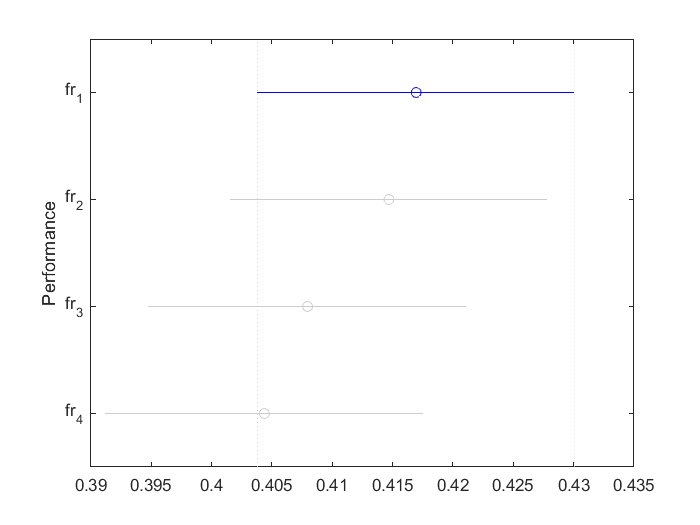
\includegraphics[width=\textwidth]{figure/heldout-ndcg-hsd.png}
	\caption{\ac{nDCG}}
     \end{subfigure}
     \hfill
     \begin{subfigure}[b]{0.45\textwidth}
         \centering
         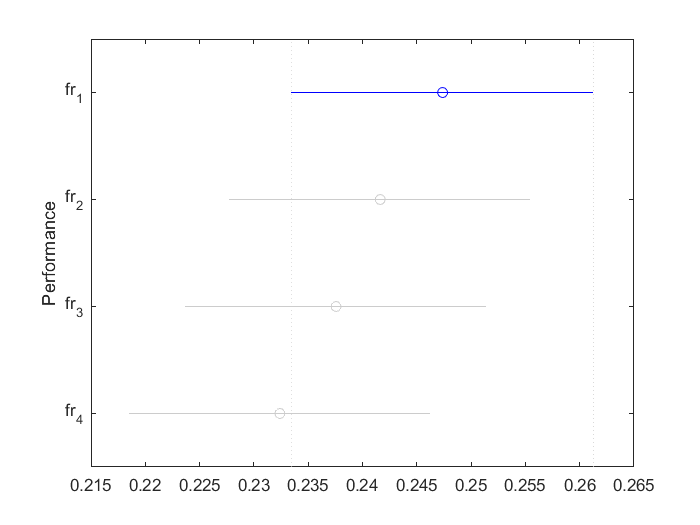
\includegraphics[width=\textwidth]{figure/heldout-map-hsd.png}
	\caption{\ac{AP}}
     \end{subfigure}
        \caption{Tukey's \ac{HSD} on heldout collection}
        \label{fig:heldout-hsd}
\end{figure}

\subsubsection{Short term}
\label{subsubsec:short-res}

In Table~\ref{tab:short-map-ndcg-table} are reported the \ac{nDCG} and \ac{MAP} values obtained from the submitted runs on the short term collection, while in Figure~\ref{fig:precision-recall-curve-short-term} is reported the interpolated Precision-Recall curve. Comparing these results with the ones obtained on heldout, shown in Table~\ref{tab:heldout-map-ndcg-table} and Figure~\ref{fig:precision-recall-curve-heldout} respectively, we can see that every run has \emph{increased} its performances. This improvement was \emph{not expected} since the performances should tend to drop over time. This can be due to the fact that this set of runs is almost 9 times bigger than the heldout, therefore we can consider the mean measures obtained to be more \emph{reliable} than the ones on the heldout collection.

Observing the \ac{nDCG} and \ac{AP} boxplots, shown in Figure~\ref{fig:short-boxplot}, we can notice that the runs performed on the French collection have a similar structure in terms of median values and interquartile ranges. We can also notice that in the \ac{AP} boxplot the fr\_1 run has a longer whisker, while the others show the presence of outliers.

From the ANOVA2 analysis, which results are reported in Table~\ref{tab:short-anova2}, we can see that $p\textrm{--}value<\alpha$, therefore we \emph{can reject} the null hypothesis. Moreover, from Tukey's \ac{HSD} multiple comparison shown in Figure~\ref{fig:short-hsd}, we can derive that runs fr\_3, fr\_4 can be considered similar, while all the other runs differ from each other.

\begin{table}[tbp]
\caption{\ac{nDCG} and \ac{MAP} values on short term collection}
  \label{tab:short-map-ndcg-table}
    \centering
    \begin{tabular}{|p{0.7\linewidth}|p{0.075\linewidth}|p{0.075\linewidth}|}
	\toprule
	\textbf{Run name} & \textbf{nDCG} & \textbf{MAP} \\
	\midrule
        FADERIC\_French-BM25-Stop50-LightStem-Shingle-Fuzzy-SynCustom-Rerank20W6 & 0.4239 & 0.2665 \\ 
        FADERIC\_French-BM25-Stop50-LightStem-Shingle-Fuzzy-Rerank30 & 0.4145 & 0.2546 \\ 
        FADERIC\_French-BM25-Stop50-LightStem-Shingle-Fuzzy-SynCustom & 0.4034 & 0.2412 \\ 
        FADERIC\_French-BM25Tuned-Stop50-LightStem-Shingle-Fuzzy & 0.4034 & 0.2414 \\ 
        FADERIC\_English-BM25-Stop50-KStem-Shingle-Fuzzy-SynPOS\\-Rerank30 & 0.3296 & 0.1931 \\ 
	\bottomrule
    \end{tabular}
\end{table}

\begin{figure}[tbp]
  \centering
  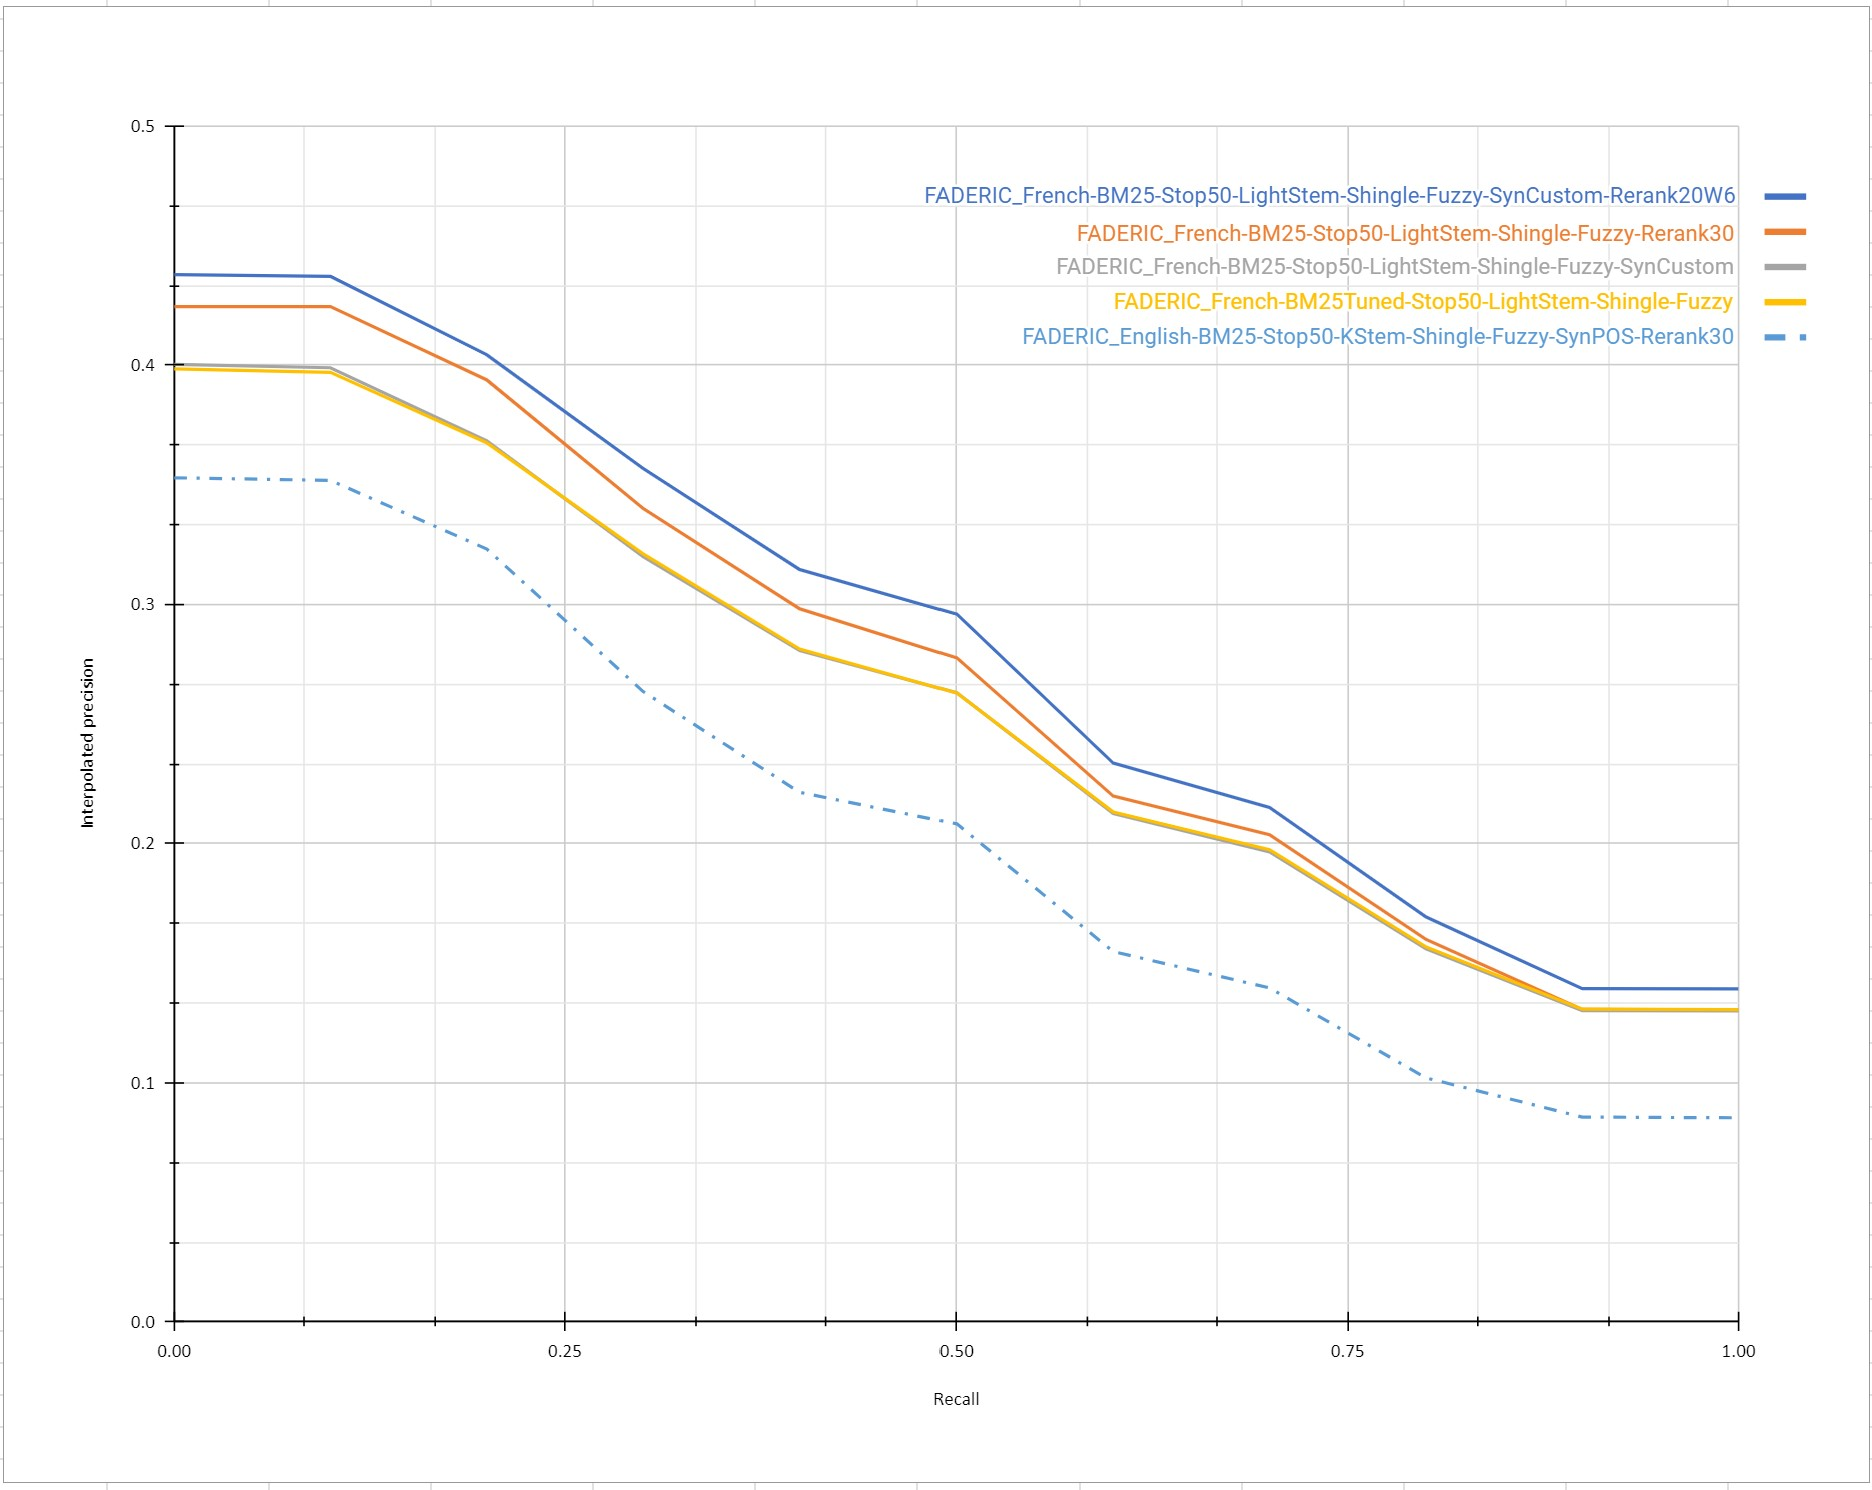
\includegraphics[width=1\linewidth]{figure/iprec-recall-SHORT-TERM.jpg}
  \caption{Interpolated Precision-Recall curve on short term collection}
  \label{fig:precision-recall-curve-short-term}
\end{figure}

\begin{figure}[tbp]
     \centering
     \begin{subfigure}[b]{0.45\textwidth}
         \centering
         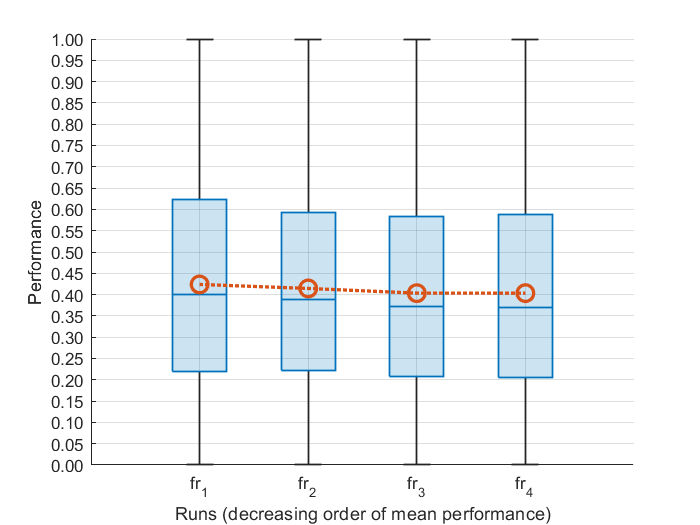
\includegraphics[width=\textwidth]{figure/short-ndcg-boxplot.png}
         \caption{\ac{nDCG}}
     \end{subfigure}
     \hfill
     \begin{subfigure}[b]{0.45\textwidth}
         \centering
         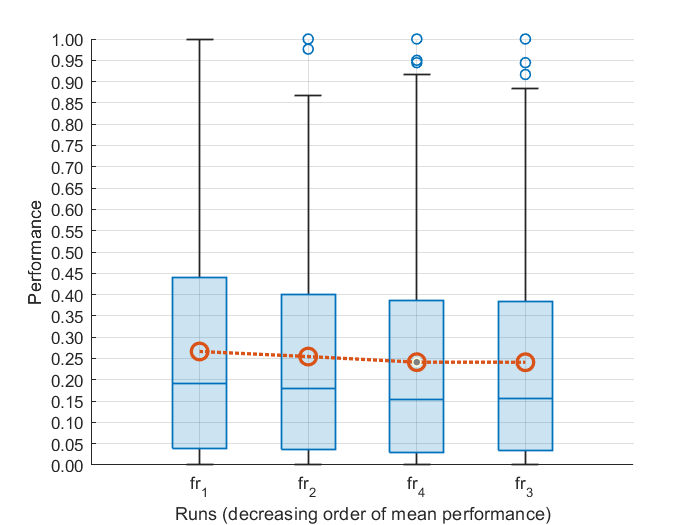
\includegraphics[width=\textwidth]{figure/short-map-boxplot.png}
         \caption{\ac{AP}}
     \end{subfigure}
        \caption{Box plot on short term collection, the mean values are shown in red}
        \label{fig:short-boxplot}
\end{figure}

\begin{table}[tbp]
     \caption{ANOVA2 on short term collection}
    \begin{subtable}[h]{1\textwidth}
        \centering
	 \caption{\ac{nDCG}}
        \begin{tabular}{|l|l|l|l|l|l|}
	\toprule
        \textbf{Source} & \textbf{SS} & \textbf{df} & \textbf{MS} & \textbf{F} & \textbf{Prob$>$F} \\
        \midrule
	\textbf{Systems} & 0.25 & 3  & 0.085  & 13.58  & 8.51E-9 \\
	\textbf{Topics}    & 218.58  & 881  & 0.248 & 39.30 & 0 \\
	\textbf{Error}   & 16.68 & 2643 & 0.006 & - & - \\
	\textbf{Total}   & 235.52  & 3527 & - & - & - \\
	\bottomrule
       \end{tabular}
    \end{subtable}
        \begin{subtable}[h]{1\textwidth}
        \centering
	\caption{\ac{AP}}
        \begin{tabular}{|l|l|l|l|l|l|}
	\toprule
        \textbf{Source} & \textbf{SS} & \textbf{df} & \textbf{MS} & \textbf{F} & \textbf{Prob$>$F} \\
        \midrule
	\textbf{Systems} & 0.38 & 3   & 0.129  & 16.05  & 2.43E-10 \\
	\textbf{Topics}    & 205.64  & 881  & 0.233 & 28.92 & 0 \\
	\textbf{Error}   & 21.32  & 2643 & 0.008 & - & - \\
	\textbf{Total}   & 227.36  & 3527 & - & - & - \\
	\bottomrule
       \end{tabular}
    \end{subtable}
     \label{tab:short-anova2}
\end{table}

\begin{figure}[tbp]
     \centering
     \begin{subfigure}[b]{0.45\textwidth}
         \centering
         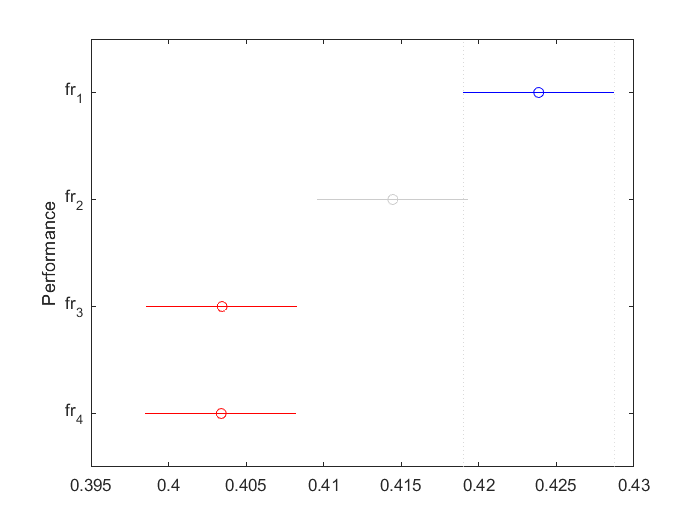
\includegraphics[width=\textwidth]{figure/short-ndcg-hsd.png}
	\caption{\ac{nDCG}}
     \end{subfigure}
     \hfill
     \begin{subfigure}[b]{0.45\textwidth}
         \centering
         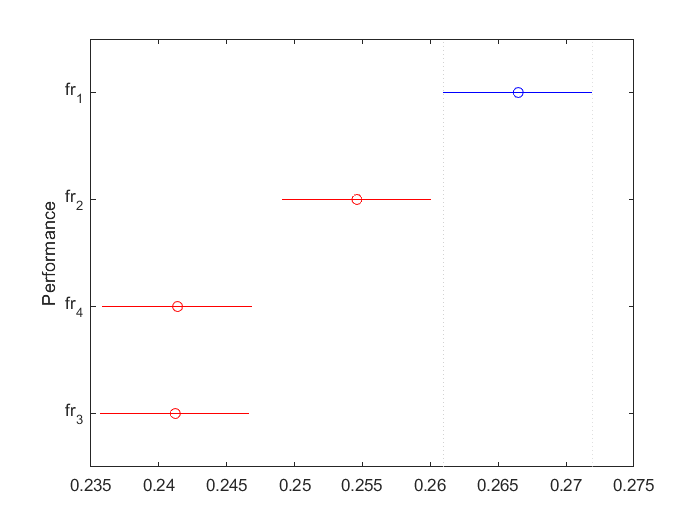
\includegraphics[width=\textwidth]{figure/short-map-hsd.png}
	\caption{\ac{AP}}
     \end{subfigure}
        \caption{Tukey's \ac{HSD} on short term collection}
        \label{fig:short-hsd}
\end{figure}

\clearpage

\subsubsection{Long term}
\label{subsubsec:long-res}

Since some error occurred in the indexing phase when performing the submitted runs fr\_1 and fr\_2, in the following analysis we will use a \emph{fixed} version of those runs.

In Table~\ref{tab:long-map-ndcg-table} are reported the \ac{nDCG} and \ac{MAP} values obtained from the submitted runs on the long term collection, while in Figure~\ref{fig:precision-recall-curve-long-term} is reported the interpolated Precision-Recall curve. Comparing these results with the ones obtained on the short term, shown in Table~\ref{tab:short-map-ndcg-table} and Figure~\ref{fig:precision-recall-curve-short-term} respectively, we can see that every run suffered a \emph{performance drop} over all the measures. This worsening was expected and it can be due to the fact that the performances tend to drop over time, however, the decrease is not huge and we can consider the performances of the system to \emph{remain satisfactory}.

Observing the \ac{nDCG} and \ac{AP} boxplots, shown in Figure~\ref{fig:long-boxplot}, we can notice that the runs performed on the French collection have a similar structure in terms of median values and interquartile ranges. We can also notice that in the \ac{AP} boxplot all the runs show the presence of outliers. 

From the ANOVA2 analysis, which results are reported in Table~\ref{tab:long-anova2}, we can see that we obtained very different results for the two measures. In particular, on \ac{nDCG} we have $p\textrm{--}value>\alpha$, which means we \emph{cannot reject} the null hypothesis, while on \ac{AP} we have $p\textrm{--}value<\alpha$, which means we \emph{can reject} the null hypothesis. The same behavior is reflected in Tukey's \ac{HSD} multiple comparison, shown in Figure~\ref{fig:long-hsd}, where on \ac{nDCG} we can derive that the French runs can be considered to be similar to each other, while on \ac{AP}  we can see that runs fr\_1, fr\_2, fr\_3 and runs fr\_3, fr\_4 can be considered similar to each other.

\begin{table}[tbp]
\caption{\ac{nDCG} and \ac{MAP} values on long term collection}
  \label{tab:long-map-ndcg-table}
    \centering
    \begin{tabular}{|p{0.7\linewidth}|p{0.075\linewidth}|p{0.075\linewidth}|}
	\toprule
	\textbf{Run name} & \textbf{nDCG} & \textbf{MAP} \\
	\midrule
        FADERIC\_French-BM25-Stop50-LightStem-Shingle-Fuzzy-SynCustom-Rerank20W6 & 0.4153 & 0.2473 \\ 
        FADERIC\_French-BM25-Stop50-LightStem-Shingle-Fuzzy-Rerank30 & 0.4146 & 0.2465 \\ 
        FADERIC\_French-BM25-Stop50-LightStem-Shingle-Fuzzy-SynCustom & 0.4091 & 0.2384 \\ 
        FADERIC\_French-BM25Tuned-Stop50-LightStem-Shingle-Fuzzy & 0.4071 & 0.2350 \\ 
        FADERIC\_English-BM25-Stop50-KStem-Shingle-Fuzzy-SynPOS\\-Rerank30 & 0.3296 & 0.1809 \\ 
	\bottomrule
    \end{tabular}
\end{table}

\begin{figure}[tbp]
  \centering
  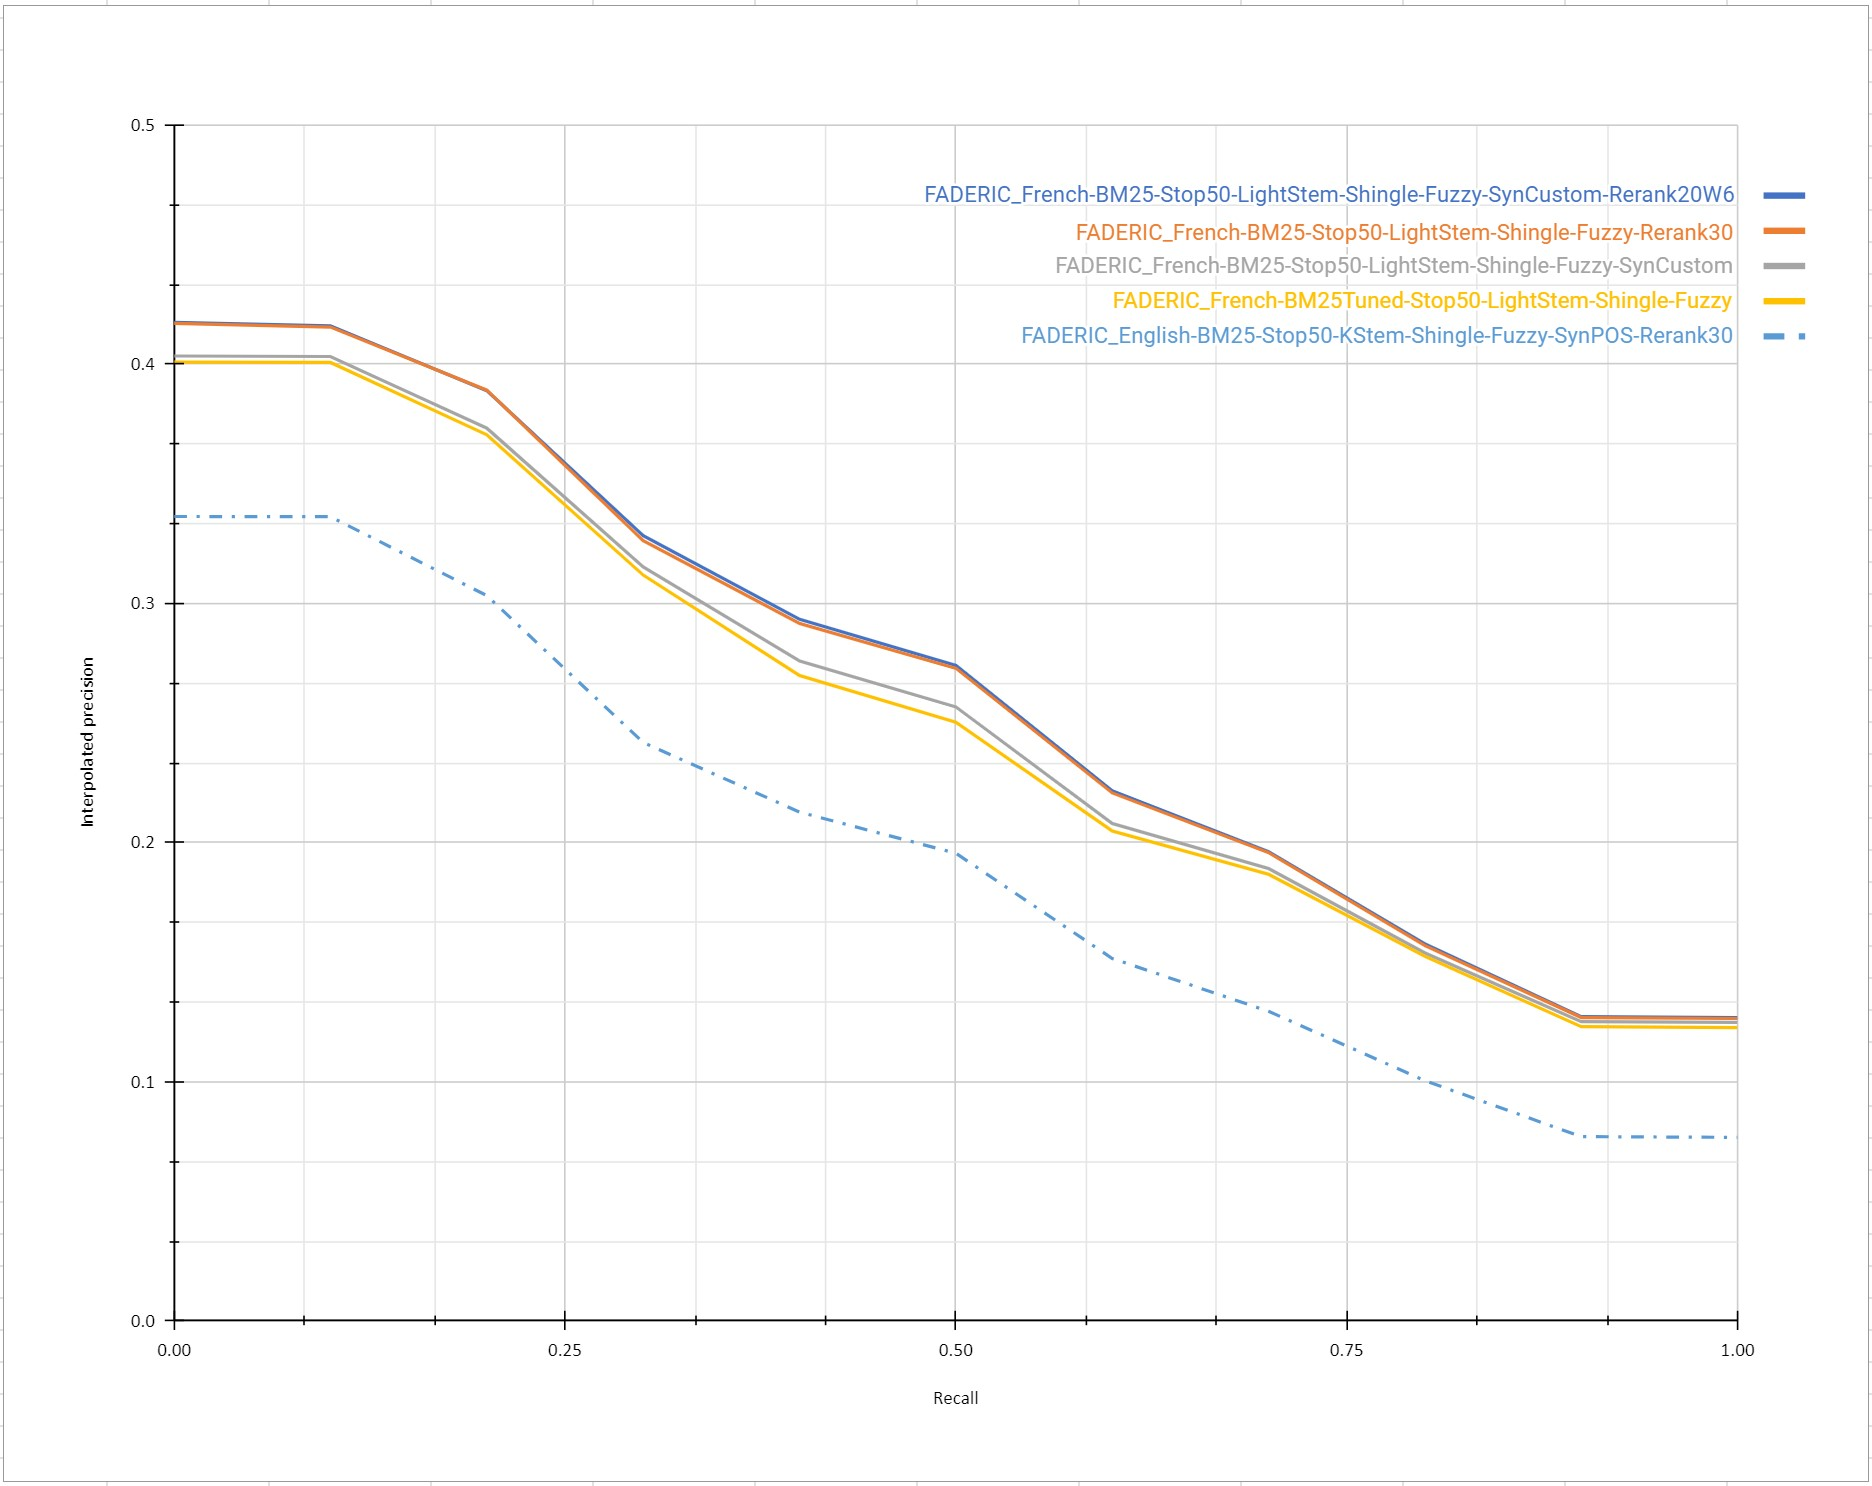
\includegraphics[width=1\linewidth]{figure/iprec-recall-LONG-TERM.jpg}
  \caption{Interpolated Precision-Recall curve on long term collection}
  \label{fig:precision-recall-curve-long-term}
\end{figure}

\begin{figure}[tbp]
     \centering
     \begin{subfigure}[b]{0.45\textwidth}
         \centering
         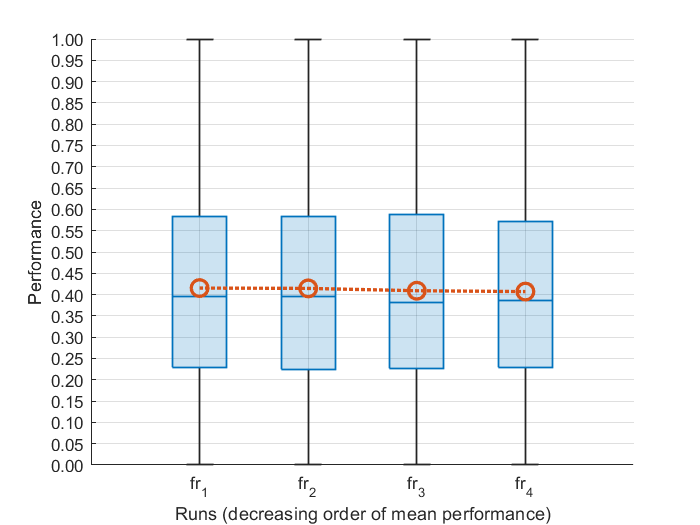
\includegraphics[width=\textwidth]{figure/long-ndcg-boxplot.png}
         \caption{\ac{nDCG}}
     \end{subfigure}
     \hfill
     \begin{subfigure}[b]{0.45\textwidth}
         \centering
         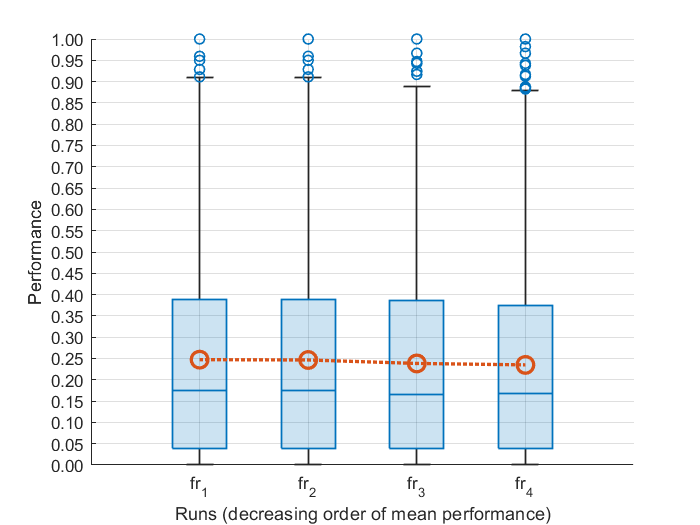
\includegraphics[width=\textwidth]{figure/long-map-boxplot.png}
         \caption{\ac{AP}}
     \end{subfigure}
        \caption{Box plot on long term collection, the mean values are shown in red}
        \label{fig:long-boxplot}
\end{figure}

\begin{table}[tbp]
     \caption{ANOVA2 on long term collection}
    \begin{subtable}[h]{1\textwidth}
        \centering
	\caption{\ac{nDCG}}
        \begin{tabular}{|l|l|l|l|l|l|}
	\toprule
        \textbf{Source} & \textbf{SS} & \textbf{df} & \textbf{MS} & \textbf{F} & \textbf{Prob$>$F} \\
        \midrule
	\textbf{Systems} & 0.04 & 3   & 0.015  & 1.51  & 0.056 \\
	\textbf{Topics}    & 202.35  & 922  & 0.219 & 16.17 & 0 \\
	\textbf{Error}   & 16.78  & 2766 & 0.006 & - & - \\
	\textbf{Total}   & 219.18  & 3691 & - & - & - \\
	\bottomrule
       \end{tabular}
    \end{subtable}
        \begin{subtable}[h]{1\textwidth}
        \centering
	\caption{\ac{AP}}
        \begin{tabular}{|l|l|l|l|l|l|}
	\toprule
        \textbf{Source} & \textbf{SS} & \textbf{df} & \textbf{MS} & \textbf{F} & \textbf{Prob$>$F} \\
        \midrule
	\textbf{Systems} & 0.10 & 3   & 0.033  & 4.47  & 0.003 \\
	\textbf{Topics}    & 188.61  & 922  & 0.204 & 27.03 & 0 \\
	\textbf{Error}   & 20.92  & 2766 & 0.007 & - & - \\
	\textbf{Total}   & 209.64  & 3691 & - & - & - \\
	\bottomrule
       \end{tabular}
    \end{subtable}
     \label{tab:long-anova2}
\end{table}

\begin{figure}[tbp]
     \centering
     \begin{subfigure}[b]{0.4\textwidth}
         \centering
         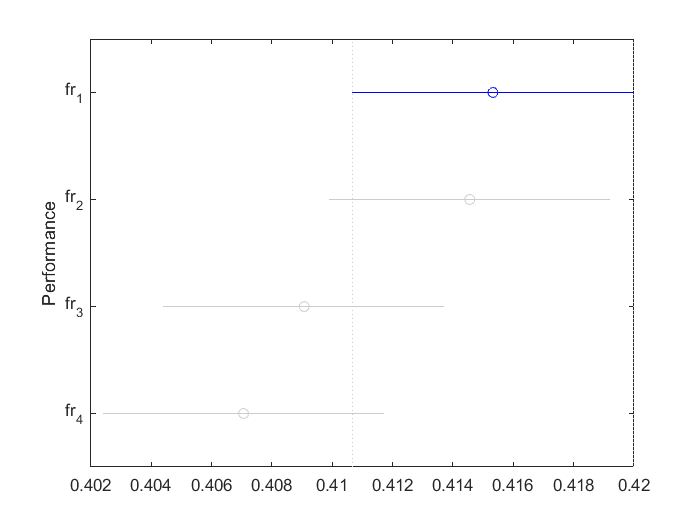
\includegraphics[width=\textwidth]{figure/long-ndcg-hsd.png}
	\caption{\ac{nDCG}}
     \end{subfigure}
     \hfill
     \begin{subfigure}[b]{0.4\textwidth}
         \centering
         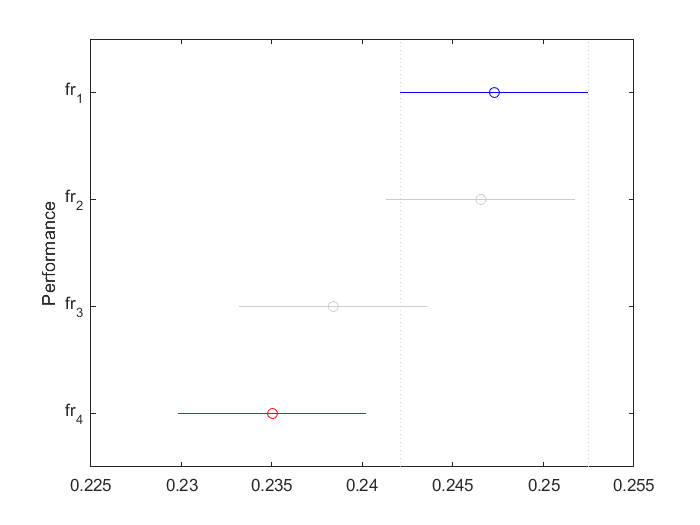
\includegraphics[width=\textwidth]{figure/long-map-hsd.png}
	\caption{\ac{AP}}
     \end{subfigure}
        \caption{Tukey's \ac{HSD} on long term collection}
        \label{fig:long-hsd}
\end{figure}

\section{Conclusions and Future Work}
\label{sec:conclusion}

From the obtained results, we can say that the system has kept \emph{satisfactory performance} from the longitudinal evaluation point of view. In fact, on the short term, there has been no significant worsening, while on the long term, there has been just a moderate performance drop.

During the developing of the system we understood that \emph{query expansion} and \emph{reranking} play a major role in the \ac{IR} systems. Those two features granted us the biggest performance improvements. Although the system has reached decent scores, our work could be  \emph{further developed} in different ways.

With respect to query expansion, we could improve the synonyms feature by using other dictionaries, since WordNet is quite outdated and a big portion of the queries were regarding very recent topics, and also by using better French dictionaries, since there are only a few available when working with languages other than English and we had to customize our own.
Another query expansion option could be switching from simple dictionaries to \emph{neural models}, in order to expand a query with words related not just to the meaning of the single words but also to the \emph{context} of the whole topic the user is looking for.

Regarding the reranker, there are some things we could improve, mainly focusing on the  \emph{trained model}. As discussed in Section~\ref{subsubsec:reranker}, we did not have the required hardware to properly train a machine learning model, so we trained on Colab with a time limit of 8 hours. This forced us to train with only 1 epoch and we tested only one set of hyperparameters, so, assuming having the necessary hardware, future improvements could focus on training a better model, with more epochs and testing different hyperparameters.
More affordable improvements could be done by dropping the libraries for training and inference and working directly with Torch for the interaction with the model, so we could be able to use the latest Torch version, which includes a new implementation of the Transformer API which speeds up training significantly.

%% Define the bibliography file to be used
\bibliography{bibliography,proceedings}

\acrodef{3G}[3G]{Third Generation Mobile System}
\acrodef{5S}[5S]{Streams, Structures, Spaces, Scenarios, Societies}
\acrodef{AA}[AA]{Active Agreements}
\acrodef{AAAI}[AAAI]{Association for the Advancement of Artificial Intelligence}
\acrodef{AAL}[AAL]{Annotation Abstraction Layer}
\acrodef{AAM}[AAM]{Automatic Annotation Manager}
\acrodef{AAP}[AAP]{Average Average Precision}
\acrodef{ACLIA}[ACLIA]{Advanced Cross-Lingual Information Access}
\acrodef{ACM}[ACM]{Association for Computing Machinery}
\acrodef{AD}[AD]{Active Disagreements}
\acrodef{ADSL}[ADSL]{Asymmetric Digital Subscriber Line}
\acrodef{ADUI}[ADUI]{ADministrator User Interface}
\acrodef{AIP}[AIP]{Archival Information Package}
\acrodef{AJAX}[AJAX]{Asynchronous JavaScript Technology and \acs{XML}}
\acrodef{ALU}[ALU]{Aritmetic-Logic Unit}
\acrodef{AMUSID}[AMUSID]{Adaptive MUSeological IDentity-service}
\acrodef{ANOVA}[ANOVA]{ANalysis Of VAriance}
\acrodef{ANSI}[ANSI]{American National Standards Institute}
\acrodef{AP}[AP]{Average Precision}
\acrodef{APC}[APC]{AP Correlation}
\acrodef{API}[API]{Application Program Interface}
\acrodef{AR}[AR]{Address Register}
\acrodef{AS}[AS]{Annotation Service}
\acrodef{ASAP}[ASAP]{Adaptable Software Architecture Performance}
\acrodef{ASI}[ASI]{Annotation Service Integrator}
\acrodef{ASL}[ASL]{Achieved Significance Level}
\acrodef{ASM}[ASM]{Annotation Storing Manager}
\acrodef{ASR}[ASR]{Automatic Speech Recognition}
\acrodef{ASUI}[ASUI]{ASsessor User Interface}
\acrodef{ATIM}[ATIM]{Annotation Textual Indexing Manager}
\acrodef{AUC}[AUC]{Area Under the ROC Curve}
\acrodef{AUI}[AUI]{Administrative User Interface}
\acrodef{AWARE}[AWARE]{Assessor-driven Weighted Averages for Retrieval Evaluation}
\acrodef{BANKS-I}[BANKS-I]{Browsing ANd Keyword Searching I}
\acrodef{BANKS-II}[BANKS-II]{Browsing ANd Keyword Searching II}
\acrodef{BH}[BH]{Benjamini-Hochberg}
\acrodef{bpref}[bpref]{Binary Preference}
\acrodef{BNF}[BNF]{Backus and Naur Form}
\acrodef{BPM}[BPM]{Bejeweled Player Model}
\acrodef{BRICKS}[BRICKS]{Building Resources for Integrated Cultural Knowledge Services}
\acrodef{CAN}[CAN]{Content Addressable Netword}
\acrodef{CAS}[CAS]{Content-And-Structure}
\acrodef{CBSD}[CBSD]{Component-Based Software Developlement}
\acrodef{CBSE}[CBSE]{Component-Based Software Engineering}
\acrodef{CB-SPE}[CB-SPE]{Component-Based \acs{SPE}}
\acrodef{CD}[CD]{Collaboration Diagram}
\acrodef{CD}[CD]{Compact Disk}
\acrodef{CDF}[CDF]{Cumulative Density Function}
\acrodef{CENL}[CENL]{Conference of European National Librarians}
\acrodef{CIDOC CRM}[CIDOC CRM]{CIDOC Conceptual Reference Model}
\acrodef{CIR}[CIR]{Current Instruction Register}
\acrodef{CIRCO}[CIRCO]{Coordinated Information Retrieval Components Orchestration}
\acrodef{CG}[CG]{Cumulated Gain}
\acrodef{CL}[CL]{Curriculum Learning}
\acrodef{CL-ESA}[CL-ESA]{Cross-Lingual Explicit Semantic Analysis}
\acrodef{CLAIRE}[CLAIRE]{Combinatorial visuaL Analytics system for Information Retrieval Evaluation}
\acrodef{CLEF1}[CLEF]{Cross-Language Evaluation Forum}
\acrodef{CLEF}[CLEF]{Conference and Labs of the Evaluation Forum}
\acrodef{CLIR}[CLIR]{Cross Language Information Retrieval}
\acrodef{CM}[CM]{Continuation Methods}
\acrodef{CMS}[CMS]{Content Management System}
\acrodef{CMT}[CMT]{Campaign Management Tool}
\acrodef{CNR}[CNR]{Italian National Council of Research}
\acrodef{CO}[CO]{Content-Only}
\acrodef{COD}[COD]{Code On Demand}
\acrodef{CODATA}[CODATA]{Committee on Data for Science and Technology}
\acrodef{COLLATE}[COLLATE]{Collaboratory for Annotation Indexing and Retrieval of Digitized Historical Archive Material}
\acrodef{CP}[CP]{Characteristic Pattern}
\acrodef{CPE}[CPE]{Control Processor Element}
\acrodef{CPU}[CPU]{Central Processing Unit}
\acrodef{CQL}[CQL]{Contextual Query Language}
\acrodef{CRP}[CRP]{Cumulated Relative Position}
\acrodef{CRUD}[CRUD]{Create--Read--Update--Delete}
\acrodef{CS}[CS]{Characteristic Structure}
\acrodef{CSM}[CSM]{Campaign Storing Manager}
\acrodef{CSS}[CSS]{Cascading Style Sheets}
\acrodef{CTR}[CTR]{Click-Through Rate}
\acrodef{CU}[CU]{Control Unit}
\acrodef{CUI}[CUI]{Client User Interface}
\acrodef{CV}[CV]{Cross-Validation}
\acrodef{DAFFODIL}[DAFFODIL]{Distributed Agents for User-Friendly Access of Digital Libraries}
\acrodef{DAO}[DAO]{Data Access Object}
\acrodef{DARE}[DARE]{Drawing Adequate REpresentations}
\acrodef{DARPA}[DARPA]{Defense Advanced Research Projects Agency}
\acrodef{DAS}[DAS]{Distributed Annotation System}
\acrodef{DB}[DB]{DataBase}
\acrodef{DBMS}[DBMS]{DataBase Management System}
\acrodef{DC}[DC]{Dublin Core}
\acrodef{DCG}[DCG]{Discounted Cumulated Gain}
\acrodef{DCMI}[DCMI]{Dublin Core Metadata Initiative}
\acrodef{DCV}[DCV]{Document Cut--off Value}
\acrodef{DD}[DD]{Deployment Diagram}
\acrodef{DDC}[DDC]{Dewey Decimal Classification}
\acrodef{DDS}[DDS]{Direct Data Structure}
\acrodef{DF}[DF]{Degrees of Freedom}
\acrodef{DFI}[DFI]{Divergence From Independence}
\acrodef{DFR}[DFR]{Divergence From Randomness}
\acrodef{DHT}[DHT]{Distributed Hash Table}
\acrodef{DI}[DI]{Digital Image}
\acrodef{DIKW}[DIKW]{Data, Information, Knowledge, Wisdom}
\acrodef{DIL}[DIL]{\acs{DIRECT} Integration Layer}
\acrodef{DiLAS}[DiLAS]{Digital Library Annotation Service}
\acrodef{DIRECT}[DIRECT]{Distributed Information Retrieval Evaluation Campaign Tool}
\acrodef{DKMS}[DKMS]{Data and Knowledge Management System}
\acrodef{DL}[DL]{Digital Library}
\acrodefplural{DL}[DL]{Digital Libraries}
\acrodef{DLMS}[DLMS]{Digital Library Management System}
\acrodef{DLOG}[DL]{Description Logics}
\acrodef{DLS}[DLS]{Digital Library System}
\acrodef{DLSS}[DLSS]{Digital Library Service System}
\acrodef{DM}[DM]{Data Mining}
\acrodef{DO}[DO]{Digital Object}
\acrodef{DOI}[DOI]{Digital Object Identifier}
\acrodef{DOM}[DOM]{Document Object Model}
\acrodef{DoMDL}[DoMDL]{Document Model for Digital Libraries}
\acrodef{DP}[DP]{Discriminative Power}
\acrodef{DPBF}[DPBF]{Dynamic Programming Best-First}
\acrodef{DR}[DR]{Data Register}
\acrodef{DRIVER}[DRIVER]{Digital Repository Infrastructure Vision for European Research}
\acrodef{DTD}[DTD]{Document Type Definition}
\acrodef{DVD}[DVD]{Digital Versatile Disk}
\acrodef{EAC-CPF}[EAC-CPF]{Encoded Archival Context for Corporate Bodies, Persons, and Families}
\acrodef{EAD}[EAD]{Encoded Archival Description}
\acrodef{EAN}[EAN]{International Article Number}
\acrodef{EBU}[EBU]{Expected Browsing Utility}
\acrodef{ECD}[ECD]{Enhanced Contenty Delivery}
\acrodef{ECDL}[ECDL]{European Conference on Research and Advanced Technology for Digital Libraries}
\acrodef{EDM}[EDM]{Europeana Data Model}
\acrodef{EG}[EG]{Execution Graph}
\acrodef{ELDA}[ELDA]{Evaluation and Language resources Distribution Agency}
\acrodef{ELRA}[ELRA]{European Language Resources Association}
\acrodef{EM}[EM]{Expectation Maximization}
\acrodef{EMMA}[EMMA]{Extensible MultiModal Annotation}
\acrodef{EPROM}[EPROM]{Erasable Programmable \acs{ROM}}
\acrodef{EQNM}[EQNM]{Extended Queueing Network Model}
\acrodef{ER}[ER]{Entity--Relationship}
\acrodef{ERR}[ERR]{Expected Reciprocal Rank}
\acrodef{ERS}[ERS]{Empirical Relational System}
\acrodef{ESA}[ESA]{Explicit Semantic Analysis}
\acrodef{ESL}[ESL]{Expected Search Length}
\acrodef{ETL}[ETL]{Extract-Transform-Load}
\acrodef{FAST}[FAST]{Flexible Annotation Service Tool}
\acrodef{FDR}[FDR]{False Discovery Rate}
\acrodef{FIFO}[FIFO]{First-In / First-Out}
\acrodef{FIRE}[FIRE]{Forum for Information Retrieval Evaluation}
\acrodef{FN}[FN]{False Negative}
\acrodef{FNR}[FNR]{False Negative Rate}
\acrodef{FOAF}[FOAF]{Friend of a Friend}
\acrodef{FORESEE}[FORESEE]{FOod REcommentation sErvER}
\acrodef{FP}[FP]{False Positive}
\acrodef{FPR}[FPR]{False Positive Rate}
\acrodef{FWER}[FWER]{Family-wise Error Rate}
\acrodef{GIF}[GIF]{Graphics Interchange Format}
\acrodef{GIR}[GIR]{Geografic Information Retrieval}
\acrodef{GAP}[GAP]{Graded Average Precision}
\acrodef{GLM}[GLM]{General Linear Model}
\acrodef{GLMM}[GLMM]{General Linear Mixed Model}
\acrodef{GMAP}[GMAP]{Geometric Mean Average Precision}
\acrodef{GoP}[GoP]{Grid of Points}
\acrodef{GPRS}[GPRS]{General Packet Radio Service}
\acrodef{gP}[gP]{Generalized Precision}
\acrodef{gR}[gR]{Generalized Recall}
\acrodef{gRBP}[gRBP]{Graded Rank-Biased Precision}
\acrodef{GT}[GT]{Generalizability Theory}
\acrodef{GTIN}[GTIN]{Global Trade Item Number}
\acrodef{GUI}[GUI]{Graphical User Interface}
\acrodef{GW}[GW]{Gateway}
\acrodef{HCI}[HCI]{Human Computer Interaction}
\acrodef{HDS}[HDS]{Hybrid Data Structure}
\acrodef{HIR}[HIR]{Hypertext Information Retrieval}
\acrodef{HIT}[HIT]{Human Intelligent Task}
\acrodef{HITS}[HITS]{Hyperlink-Induced Topic Search}
\acrodef{HMM}[HMM]{Hidden Markov Model}
\acrodef{HTML}[HTML]{HyperText Markup Language}
\acrodef{HTTP}[HTTP]{HyperText Transfer Protocol}
\acrodef{HSD}[HSD]{Honestly Significant Difference}
\acrodef{ICA}[ICA]{International Council on Archives}
\acrodef{ICSU}[ICSU]{International Council for Science}
\acrodef{IDF}[IDF]{Inverse Document Frequency}
\acrodef{IDS}[IDS]{Inverse Data Structure}
\acrodef{IEEE}[IEEE]{Institute of Electrical and Electronics Engineers}
\acrodef{IEI}[IEI]{Istituto della Enciclopedia Italiana fondata da Giovanni Treccani}
\acrodef{IETF}[IETF]{Internet Engineering Task Force}
\acrodef{IIR}[IIR]{Interactive Information Retrieval}
\acrodef{IMS}[IMS]{Information Management System}
\acrodef{IMSPD}[IMS]{Information Management Systems Research Group}
\acrodef{indAP}[indAP]{Induced Average Precision}
\acrodef{infAP}[infAP]{Inferred Average Precision}
\acrodef{INEX}[INEX]{INitiative for the Evaluation of \acs{XML} Retrieval}
\acrodef{INS-M}[INS-M]{Inverse Set Data Model}
\acrodef{INTR}[INTR]{Interrupt Register}
\acrodef{IP}[IP]{Internet Protocol}
\acrodef{IPSA}[IPSA]{Imaginum Patavinae Scientiae Archivum}
\acrodef{IR}[IR]{Information Retrieval}
\acrodef{IRON}[IRON]{Information Retrieval ON}
\acrodef{IRON2}[IRON$^2$]{Information Retrieval On aNNotations}
\acrodef{IRON-SAT}[IRON-SAT]{\acs{IRON} - Statistical Analysis Tool}
\acrodef{IRS}[IRS]{Information Retrieval System}
\acrodef{ISAD(G)}[ISAD(G)]{International Standard for Archival Description (General)}
\acrodef{ISBN}[ISBN]{International Standard Book Number}
\acrodef{ISIS}[ISIS]{Interactive SImilarity Search}
\acrodef{ISJ}[ISJ]{Interactive Searching and Judging}
\acrodef{ISO}[ISO]{International Organization for Standardization}
\acrodef{ITU}[ITU]{International Telecommunication Union }
\acrodef{ITU-T}[ITU-T]{Telecommunication Standardization Sector of \acs{ITU}}
\acrodef{IV}[IV]{Information Visualization}
\acrodef{JAN}[JAN]{Japanese Article Number}
\acrodef{JDBC}[JDBC]{Java DataBase Connectivity}
\acrodef{JMB}[JMB]{Java--Matlab Bridge}
\acrodef{JNI}[JNI]{Java Native Interface}
\acrodef{JPEG}[JPEG]{Joint Photographic Experts Group}
\acrodef{JSON}[JSON]{JavaScript Object Notation}
\acrodef{JSP}[JSP]{Java Server Pages}
\acrodef{JTE}[JTE]{Java-Treceval Engine}
\acrodef{JVM}[JVM]{Java Virtual Machine}
\acrodef{KDE}[KDE]{Kernel Density Estimation}
\acrodef{KLD}[KLD]{Kullback-Leibler Divergence}
\acrodef{KLAPER}[KLAPER]{Kernel LAnguage for PErformance and Reliability analysis}
\acrodef{LAM}[LAM]{Libraries, Archives, and Museums}
\acrodef{LAM2}[LAM]{Logistic Average Misclassification}
\acrodef{LAN}[LAN]{Local Area Network}
\acrodef{LD}[LD]{Linked Data}
\acrodef{LEAF}[LEAF]{Linking and Exploring Authority Files}
\acrodef{LIDO}[LIDO]{Lightweight Information Describing Objects}
\acrodef{LIFO}[LIFO]{Last-In / First-Out}
\acrodef{LM}[LM]{Language Model}
\acrodef{LMT}[LMT]{Log Management Tool}
\acrodef{LOD}[LOD]{Linked Open Data}
\acrodef{LODE}[LODE]{Linking Open Descriptions of Events}
\acrodef{LpO}[LpO]{Leave-$p$-Out}
\acrodef{LRM}[LRM]{Local Relational Model}
\acrodef{LRU}[LRU]{Last Recently Used}
\acrodef{LS}[LS]{Lexical Signature}
\acrodef{LSM}[LSM]{Log Storing Manager}
\acrodef{LtR}[LtR]{Learning to Rank}
\acrodef{LUG}[LUG]{Lexical Unit Generator}
\acrodef{MA}[MA]{Mobile Agent}
\acrodef{MA}[MA]{Moving Average}
\acrodef{MACS}[MACS]{Multilingual ACcess to Subjects}
\acrodef{MADCOW}[MADCOW]{Multimedia Annotation of Digital Content Over the Web}
\acrodef{MAD}[MAD]{Mean Assessed Documents}
\acrodef{MADP}[MADP]{Mean Assessed Documents Precision}
\acrodef{MADS}[MADS]{Metadata Authority Description Standard}
\acrodef{MAP}[MAP]{Mean Average Precision}
\acrodef{MARC}[MARC]{Machine Readable Cataloging}
\acrodef{MATTERS}[MATTERS]{MATlab Toolkit for Evaluation of information Retrieval Systems}
\acrodef{MDA}[MDA]{Model Driven Architecture}
\acrodef{MDD}[MDD]{Model-Driven Development}
\acrodef{METS}[METS]{Metadata Encoding and Transmission Standard}
\acrodef{MIDI}[MIDI]{Musical Instrument Digital Interface}
\acrodef{MIME}[MIME]{Multipurpose Internet Mail Extensions}
\acrodef{ML}[ML]{Machine Learning}
\acrodef{MLE}[MLE]{Maximum Likelihood Estimation}
\acrodef{MLIA}[MLIA]{MultiLingual Information Access}
\acrodef{MM}[MM]{Machinery Model}
\acrodef{MMU}[MMU]{Memory Management Unit}
\acrodef{MODS}[MODS]{Metadata Object Description Schema}
\acrodef{MOF}[MOF]{Meta-Object Facility}
\acrodef{MP}[MP]{Markov Precision}
\acrodef{MPEG}[MPEG]{Motion Picture Experts Group}
\acrodef{MRD}[MRD]{Machine Readable Dictionary}
\acrodef{MRF}[MRF]{Markov Random Field}
\acrodef{MRR}[MRR]{Mean Reciprocal Rank}
\acrodef{MS}[MS]{Mean Squares}
\acrodef{MSAC}[MSAC]{Multilingual Subject Access to Catalogues}
\acrodef{MSE}[MSE]{Mean Square Error}
\acrodef{MT}[MT]{Machine Translation}
\acrodef{MV}[MV]{Majority Vote}
\acrodef{MVC}[MVC]{Model-View-Controller}
\acrodef{NACSIS}[NACSIS]{NAtional Center for Science Information Systems}
\acrodef{NAP}[NAP]{Network processors Applications Profile}
\acrodef{NCP}[NCP]{Normalized Cumulative Precision}
\acrodef{nCG}[nCG]{Normalized Cumulated Gain}
\acrodef{nCRP}[nCRP]{Normalized Cumulated Relative Position}
\acrodef{nDCG}[nDCG]{Normalized Discounted Cumulated Gain}
\acrodef{nMCG}[nMCG]{Normalized Markov Cumulated Gain}
\acrodef{NESTOR}[NESTOR]{NEsted SeTs for Object hieRarchies}
\acrodef{NEXI}[NEXI]{Narrowed Extended XPath I}
\acrodef{NII}[NII]{National Institute of Informatics}
\acrodef{NISO}[NISO]{National Information Standards Organization}
\acrodef{NIST}[NIST]{National Institute of Standards and Technology}
\acrodef{NLP}[NLP]{Natural Language Processing}
\acrodef{NN}[NN]{Neural Network}
\acrodef{NP}[NP]{Network Processor}
\acrodef{NR}[NR]{Normalized Recall}
\acrodef{NRS}[NRS]{Numerical Relational System}
\acrodef{NS-M}[NS-M]{Nested Set Model}
\acrodef{NTCIR}[NTCIR]{NII Testbeds and Community for Information access Research}
\acrodef{OAI}[OAI]{Open Archives Initiative}
\acrodef{OAI-ORE}[OAI-ORE]{Open Archives Initiative Object Reuse and Exchange}
\acrodef{OAI-PMH}[OAI-PMH]{Open Archives Initiative Protocol for Metadata Harvesting}
\acrodef{OAIS}[OAIS]{Open Archival Information System}
\acrodef{OC}[OC]{Operation Code}
\acrodef{OCLC}[OCLC]{Online Computer Library Center}
\acrodef{OMG}[OMG]{Object Management Group}
\acrodef{OO}[OO]{Object Oriented}
\acrodef{OODB}[OODB]{Object-Oriented \acs{DB}}
\acrodef{OODBMS}[OODBMS]{Object-Oriented \acs{DBMS}}
\acrodef{OPAC}[OPAC]{Online Public Access Catalog}
\acrodef{OQL}[OQL]{Object Query Language}
\acrodef{ORP}[ORP]{Open Relevance Project}
\acrodef{OSIRIS}[OSIRIS]{Open Service Infrastructure for Reliable and Integrated process Support}
\acrodef{P}[P]{Precision}
\acrodef{P2P}[P2P]{Peer-To-Peer}
\acrodef{PA}[PA]{Passive Agreements}
\acrodef{PAMT}[PAMT]{Pool-Assessment Management Tool}
\acrodef{PASM}[PASM]{Pool-Assessment Storing Manager}
\acrodef{PC}[PC]{Program Counter}
\acrodef{PCP}[PCP]{Pre-Commercial Procurement}
\acrodef{PCR}[PCR]{Peripherical Command Register}
\acrodef{PD}[PD]{Passive Disagreements}
\acrodef{PDA}[PDA]{Personal Digital Assistant}
\acrodef{PDF}[PDF]{Probability Density Function}
\acrodef{PDR}[PDR]{Peripherical Data Register}
\acrodef{PIR}[PIR]{Personalized Information Retrieval}
\acrodef{POI}[POI]{\acs{PURL}-based Object Identifier}
\acrodef{PoS}[PoS]{Part of Speech}
\acrodef{PAA}[PAA]{Proportion of Active Agreements}
\acrodef{PPA}[PPA]{Proportion of Passive Agreements}
\acrodef{PPE}[PPE]{Programmable Processing Engine}
\acrodef{PREFORMA}[PREFORMA]{PREservation FORMAts for culture information/e-archives}
\acrodef{PRIMAD}[PRIMAD]{Platform, Research goal, Implementation, Method, Actor, and Data}
\acrodef{PRIMAmob-UML}[PRIMAmob-UML]{mobile \acs{PRIMA-UML}}
\acrodef{PRIMA-UML}[PRIMA-UML]{PeRformance IncreMental vAlidation in \acs{UML}}
\acrodef{PROM}[PROM]{Programmable \acs{ROM}}
\acrodef{PROMISE}[PROMISE]{Participative Research labOratory  for Multimedia and Multilingual Information Systems Evaluation}
\acrodef{pSQL}[pSQL]{propagate \acs{SQL}}
\acrodef{PUI}[PUI]{Participant User Interface}
\acrodef{PURL}[PURL]{Persistent \acs{URL}}
\acrodef{QA}[QA]{Question Answering}
\acrodef{QE}[QE]{Query Expansion}
\acrodef{QoS-UML}[QoS-UML]{\acs{UML} Profile for QoS and Fault Tolerance}
\acrodef{QPA}[QPA]{Query Performance Analyzer}
\acrodef{QPP}[QPP]{Query Performance Prediction}
\acrodef{R}[R]{Recall}
\acrodef{RAM}[RAM]{Random Access Memory}
\acrodef{RAMM}[RAM]{Random Access Machine}
\acrodef{RBO}[RBO]{Rank-Biased Overlap}
\acrodef{RBP}[RBP]{Rank-Biased Precision}
\acrodef{RBTO}[RBTO]{Rank-Based Total Order}
\acrodef{RDBMS}[RDBMS]{Relational \acs{DBMS}}
\acrodef{RDF}[RDF]{Resource Description Framework}
\acrodef{REST}[REST]{REpresentational State Transfer}
\acrodef{REV}[REV]{Remote Evaluation}
\acrodef{RF}[RF]{Relevance Feedback}
\acrodef{RFC}[RFC]{Request for Comments}
\acrodef{RIA}[RIA]{Reliable Information Access}
\acrodef{RMSE}[RMSE]{Root Mean Square Error}
\acrodef{RMT}[RMT]{Run Management Tool}
\acrodef{ROM}[ROM]{Read Only Memory}
\acrodef{ROMIP}[ROMIP]{Russian Information Retrieval Evaluation Seminar}
\acrodef{RoMP}[RoMP]{Rankings of Measure Pairs}
\acrodef{RoS}[RoS]{Rankings of Systems}
\acrodef{RP}[RP]{Relative Position}
\acrodef{RR}[RR]{Reciprocal Rank}
\acrodef{RSM}[RSM]{Run Storing Manager}
\acrodef{RST}[RST]{Rhetorical Structure Theory}
\acrodef{RSV}[RSV]{Retrieval Status Value}
\acrodef{RT-UML}[RT-UML]{\acs{UML} Profile for Schedulability, Performance and Time}
\acrodef{SA}[SA]{Software Architecture}
\acrodef{SAL}[SAL]{Storing Abstraction Layer}
\acrodef{SAMT}[SAMT]{Statistical Analysis Management Tool}
\acrodef{SAN}[SAN]{Sistema Archivistico Nazionale}
\acrodef{SASM}[SASM]{Statistical Analysis Storing Manager}
\acrodef{SBTO}[SBTO]{Set-Based Total Order}
\acrodef{SD}[SD]{Sequence Diagram}
\acrodef{SE}[SE]{Search Engine}
\acrodef{SEBD}[SEBD]{Convegno Nazionale su Sistemi Evoluti per Basi di Dati}
\acrodef{SEM}[SEM]{Standard Error of the Mean}
\acrodef{SERP}[SERP]{Search Engine Result Page}
\acrodef{SFT}[SFT]{Satisfaction--Frustration--Total}
\acrodef{SIL}[SIL]{Service Integration Layer}
\acrodef{SIP}[SIP]{Submission Information Package}
\acrodef{SKOS}[SKOS]{Simple Knowledge Organization System}
\acrodef{SM}[SM]{Software Model}
\acrodef{SME}[SME]{Statistics--Metrics-Experiments}
\acrodef{SMART}[SMART]{System for the Mechanical Analysis and Retrieval of Text}
\acrodef{SoA}[SoA]{Service-oriented Architectures}
\acrodef{SOA}[SOA]{Strength of Association}
\acrodef{SOAP}[SOAP]{Simple Object Access Protocol}
\acrodef{SOM}[SOM]{Self-Organizing Map}
\acrodef{SPARQL}[SPARQL]{Simple Protocol and RDF Query Language}
\acrodef{SPE}[SPE]{Software Performance Engineering}
\acrodef{SPINA}[SPINA]{Superimposed Peer Infrastructure for iNformation Access}
\acrodef{SPLIT}[SPLIT]{Stemming Program for Language Independent Tasks}
\acrodef{SPOOL}[SPOOL]{Simultaneous Peripheral Operations On Line}
\acrodef{SQL}[SQL]{Structured Query Language}
\acrodef{SR}[SR]{Sliding Ratio}
\acrodef{sRBP}[sRBP]{Session Rank Biased Precision}
\acrodef{SRU}[SRU]{Search/Retrieve via \acs{URL}}
\acrodef{SS}[SS]{Sum of Squares}
\acrodef{SSD}[s.s.d.]{statistically significantly different}
\acrodef{SSTF}[SSTF]{Shortest Seek Time First}
\acrodef{STAR}[STAR]{Steiner-Tree Approximation in Relationship graphs}
\acrodef{STON}[STON]{STemming ON}
\acrodef{SVM}[SVM]{Support Vector Machine}
\acrodef{TAC}[TAC]{Text Analysis Conference}
\acrodef{TBG}[TBG]{Time-Biased Gain}
\acrodef{TCP}[TCP]{Transmission Control Protocol}
\acrodef{TEL}[TEL]{The European Library}
\acrodef{TERRIER}[TERRIER]{TERabyte RetrIEveR}
\acrodef{TF}[TF]{Term Frequency}
\acrodef{TFR}[TFR]{True False Rate}
\acrodef{TLD}[TLD]{Top Level Domain}
\acrodef{TME}[TME]{Topics--Metrics-Experiments}
\acrodef{TN}[TN]{True Negative}
\acrodef{TO}[TO]{Transfer Object}
\acrodef{TP}[TP]{True Positve}
\acrodef{TPR}[TPR]{True Positive Rate}
\acrodef{TRAT}[TRAT]{Text Relevance Assessing Task}
\acrodef{TREC}[TREC]{Text REtrieval Conference}
\acrodef{TRECVID}[TRECVID]{TREC Video Retrieval Evaluation}
\acrodef{TTL}[TTL]{Time-To-Live}
\acrodef{UCD}[UCD]{Use Case Diagram}
\acrodef{UDC}[UDC]{Universal Decimal Classification}
\acrodef{uGAP}[uGAP]{User-oriented Graded Average Precision}
\acrodef{UI}[UI]{User Interface}
\acrodef{UML}[UML]{Unified Modeling Language}
\acrodef{UMT}[UMT]{User Management Tool}
\acrodef{UMTS}[UMTS]{Universal Mobile Telecommunication System}
\acrodef{UoM}[UoM]{Utility-oriented Measurement}
\acrodef{UPC}[UPC]{Universal Product Code}
\acrodef{URI}[URI]{Uniform Resource Identifier}
\acrodef{URL}[URL]{Uniform Resource Locator}
\acrodef{URN}[URN]{Uniform Resource Name}
\acrodef{USM}[USM]{User Storing Manager}
\acrodef{VA}[VA]{Visual Analytics}
\acrodef{VAIRE}[VAIR\"{E}]{Visual Analytics for Information Retrieval Evaluation}
\acrodef{VATE}[VATE$^2$]{Visual Analytics Tool for Experimental Evaluation}
\acrodef{VIRTUE}[VIRTUE]{Visual Information Retrieval Tool for Upfront Evaluation}
\acrodef{VD}[VD]{Virtual Document}
\acrodef{VDM}[VDM]{Visual Data Mining}
\acrodef{VIAF}[VIAF]{Virtual International Authority File}
\acrodef{VIM}[VIM]{International Vocabulary of Metrology}
\acrodef{VL}[VL]{Visual Language}
\acrodef{VoIP}[VoIP]{Voice over IP}
\acrodef{VS}[VS]{Visual Sentence}
\acrodef{W3C}[W3C]{World Wide Web Consortium}
\acrodef{WAN}[WAN]{Wide Area Network}
\acrodef{WHO}[WHO]{World Health Organization}
\acrodef{WLAN}[WLAN]{Wireless \acs{LAN}}
\acrodef{WP}[WP]{Work Package}
\acrodef{WS}[WS]{Web Services}
\acrodef{WSD}[WSD]{Word Sense Disambiguation}
\acrodef{WSDL}[WSDL]{Web Services Description Language}
\acrodef{WWW}[WWW]{World Wide Web}
\acrodef{XMI}[XMI]{\acs{XML} Metadata Interchange}
\acrodef{XML}[XML]{eXtensible Markup Language}
\acrodef{XPath}[XPath]{XML Path Language}
\acrodef{XSL}[XSL]{eXtensible Stylesheet Language}
\acrodef{XSL-FO}[XSL-FO]{\acs{XSL} Formatting Objects}
\acrodef{XSLT}[XSLT]{\acs{XSL} Transformations}
\acrodef{YAGO}[YAGO]{Yet Another Great Ontology}
\acrodef{YASS}[YASS]{Yet Another Suffix Stripper}


\end{document}
